\section{Page--Wootters and detector models for a three-level system}
\label{sec:pw3l}\label{sec:pw:apps_last}

A two-level system is the simplest non-trivial quantum system and,
as seen in Sec.~\ref{sec:absorption+pw},
it is sufficient to illustrate
models of quantum time of arrival,
such as those based on complex potentials,
as well as relational models.
Therein, numerical examples have been shown, where the two approaches
---discrete Page--Wootters and the ``non Hermitian'' detector models---
lead to
compatible predictions.

A three-level atom (or a three-level quantum system in general) appears
naturally
as
the next computational step;
but far from being merely another exercise
---just at a slightly higher level of complexity
but otherwise showing, essentially, the same physics---
it is in fact the \emph{minimal} system \emph{required}
to realize a broad
phenomenology that includes the
\term{Stimulated Raman adiabatic passage}
---STIRAP \parencite{Ruschhaupt_AtomDiode, NonHermitianShortcutSTIRAP, OptimizedTransferSTIRAP, Ruschhaupt_STA23}
and the
\term{Electromagnetically induced transparency}
---EIT \parencite{EIT_Review}.

% Also, it is shown that a three-level atom can model
% a more robust and realistic
% detector for time-of-arrival measurement, compared to the one implemented
% with a two-level atom (as introduced in Sec.~\ref{sec:hist:detect}).
% The atom can be ``driven'' by a laser
% from the ground state $\ket{0}$ into the excited state $\ket{2}$,
% then decay into a metastable state $\ket{1}$ at an intermediate energy
% (see the above references, although they might use a slightly different notation).
% This prevents the atom from decaying again and altering the ``arrival'' detection.

As usual, we are going to set $\hbar = 1$ in the following numerical computation,
based, once again, on the
\emph{NumPy} framework \parencite{comp:numpy},
within a
\term{Jupyter notebook} \parencite{comp:jupyter}.
Details can be consulted in the Appendix~\ref{detector-model-3-level-system}.
Full source code is available from the repository at ref. \cite{OwnJupyterRepo}.

\subsection{Hermitian evolution}

In our numerical example, the following
Hamiltonian is considered:
\begin{equation}\label{eq:3lev:H}
  H \repr \frac{1}{96} \mqty(
    -2  & 0 & 32  \\
     0  & 2 & 8   \\
    32  & 8 & 3
  )
  \text{,}
\end{equation}
with respect to the
%fiducial
basis $\qty{\ket{0}, \ket{1}, \ket{2}}$.
Let also
the initial state be $\ket{\psi(0)} = \ket{0} \repr \mqty(1 \\ 0 \\ 0)$.

The system will evolve \emph{unitarily}, according to $\ket{\psi(t)} = \E^{-\iu H t} \ket{\psi(0)}$,
which is computed numerically:
\begin{lstlisting}[language=Python]
import numpy as np
from scipy.linalg import expm, norm

H = np.array([
  [-2,     0,      32],
  [0,      2,       8],
  [32,     8,       3]
], np.complex_) / 96

psi_0 = np.array([1, 0, 0], np.complex_)

def U(t):
    return expm(-1j*H*t)

def unitary_psi(t):
    return U(t) @ psi_0
\end{lstlisting}

We are interested in the probability of the system to be in $\ket{0}$, $\ket{1}$, or $\ket{2}$,
which is given by $\abs{\braket{0, 1, 2}{\psi(t)}}^2$:
\begin{lstlisting}[language=Python]
def prob(t):
  probabilities = [0, 0, 0]
  for i in 0, 1, 2:
      probabilities[i] = norm(unitary_psi(t)[i])**2
      return probabilities
\end{lstlisting}
Such probabilities over time are shown in Figure \ref{fig:3lev:probs}. 

\begin{figure}[]
  \begin{subfigure}[b]{\textwidth}
    \centering
    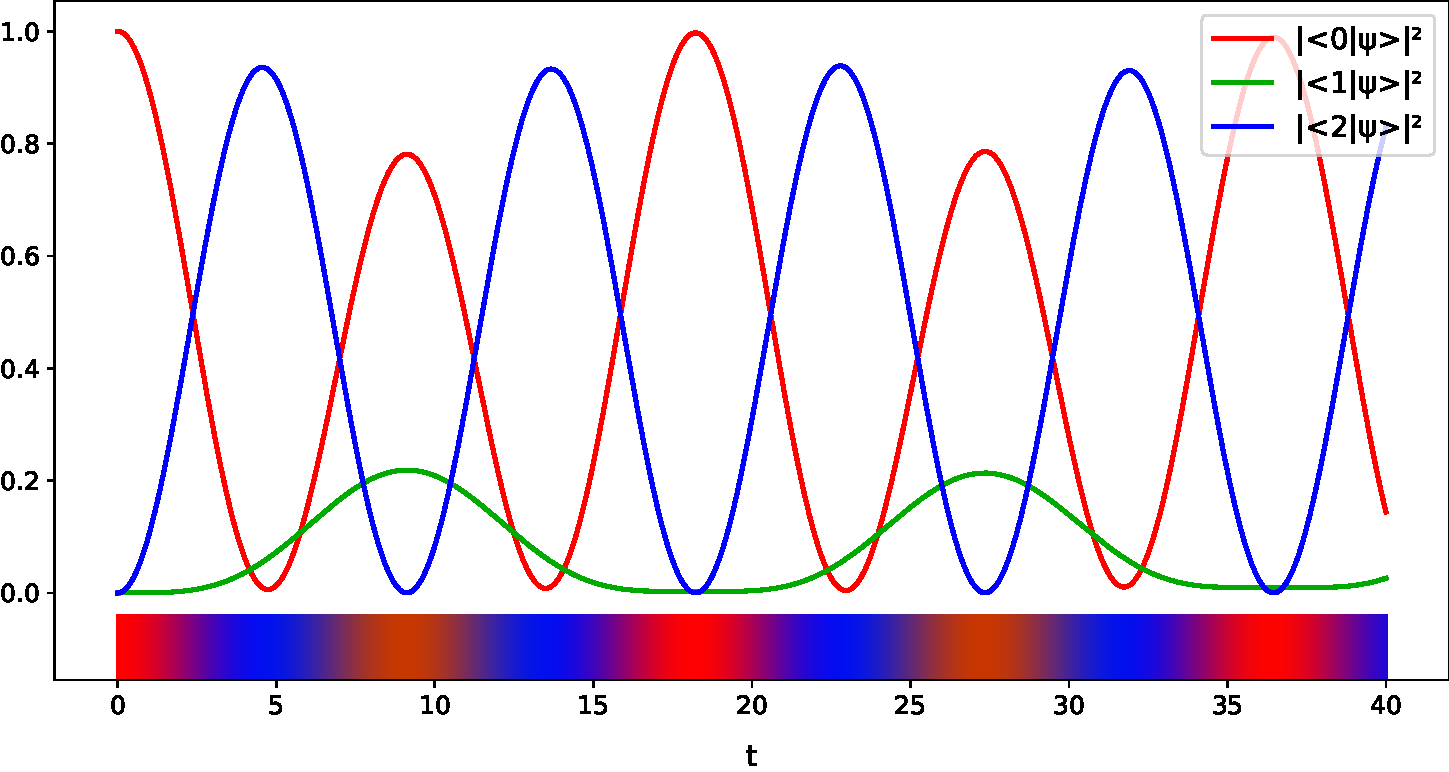
\includegraphics[width=.8\textwidth]{img/3ldetect/hermitian3lines.pdf}
    \subcaption{
      Probabilities for the three-level system.
      \emph{Note}:
        a three-level system allows a graphical representation
        where primary colors can be combined
        (see the bar at the bottom) to immediately
        visualize which probability dominates.
    }
    \label{fig:3lev:probs:lines}
  \end{subfigure}
  \par\bigskip
  \par\bigskip
  \begin{subfigure}[b]{\textwidth}
    \centering
    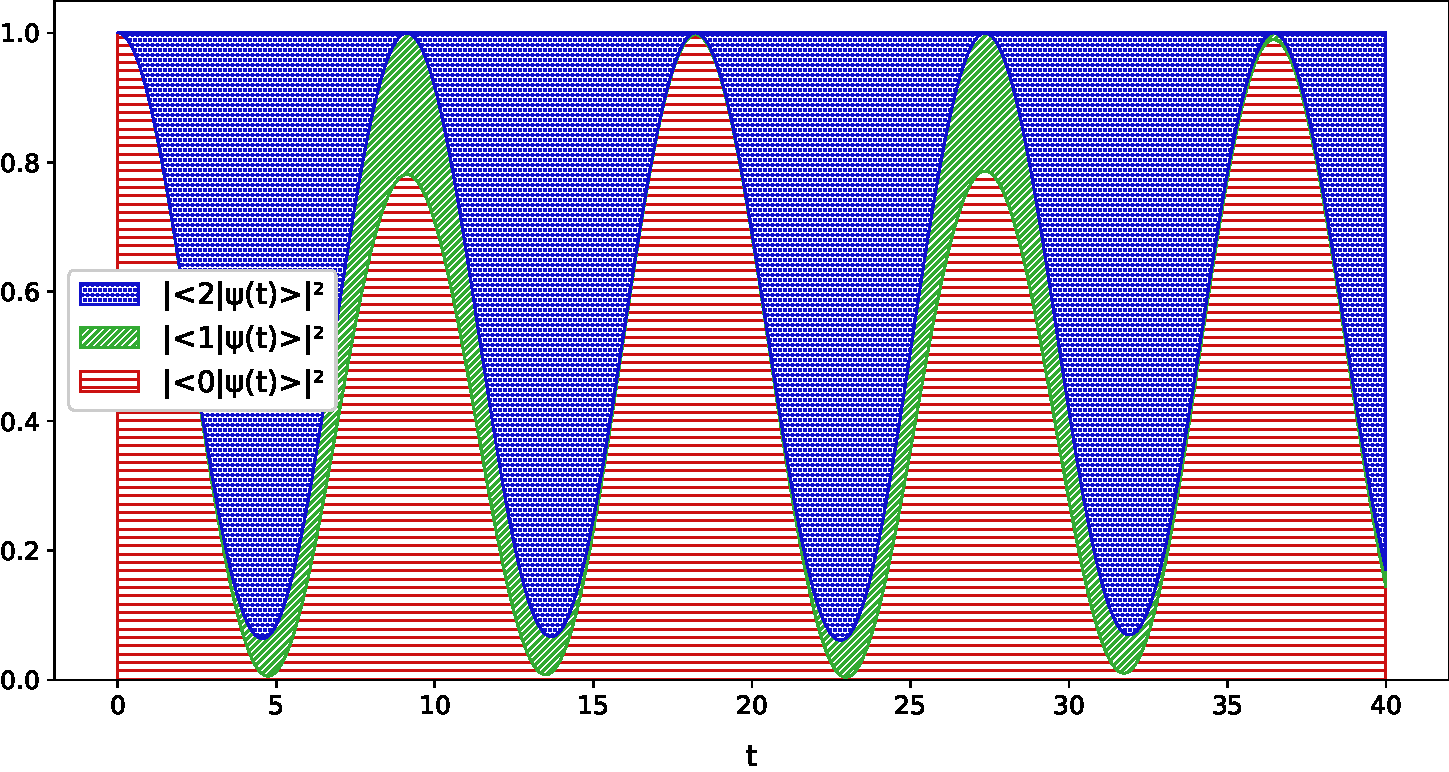
\includegraphics[width=.8\textwidth]{img/3ldetect/hermitian3color.pdf}
    \subcaption{\setstretch{1.25}
      \emph{Stacked} probability chart shows that their sum
      $\sum_{i=0}^{2} \abs{\braket{i}{\psi(t)}}^2$
      is constantly equal to 1 at any time $t$.
      That is equal to the norm $\norm{\psi(t)}^2$, which is indeed conserved
      as
      the system evolves \emph{unitarily}.
    }
    \label{fig:3lev:probs:stack}
  \end{subfigure}
  \par\bigskip
  \par\bigskip
  \caption{
    Probabilities
      $\abs{\braket{i}{\psi(t)}}^2$ for $i \in \qty{0, 1, 2}.$
  }
  \label{fig:3lev:probs}
\end{figure}

We are also interested in probability \term{amplitudes}:
complex values of
$\braket{0}{\psi(t)}$, 
$\braket{1}{\psi(t)}$, and
$\braket{2}{\psi(t)}$
are represented in the three-dimensional
plot in Fig.~\ref{fig:3lev:hermitianEvol}.
Once again, the two horizontal axes are used for the real and imaginary part of
$\braket{0, 1, 2}{\psi(t)}$,
while the independent variable $t$ (time) is represented on the vertical axis.
\begin{figure}[]
  \begin{subfigure}[t]{\textwidth}
    \centering
    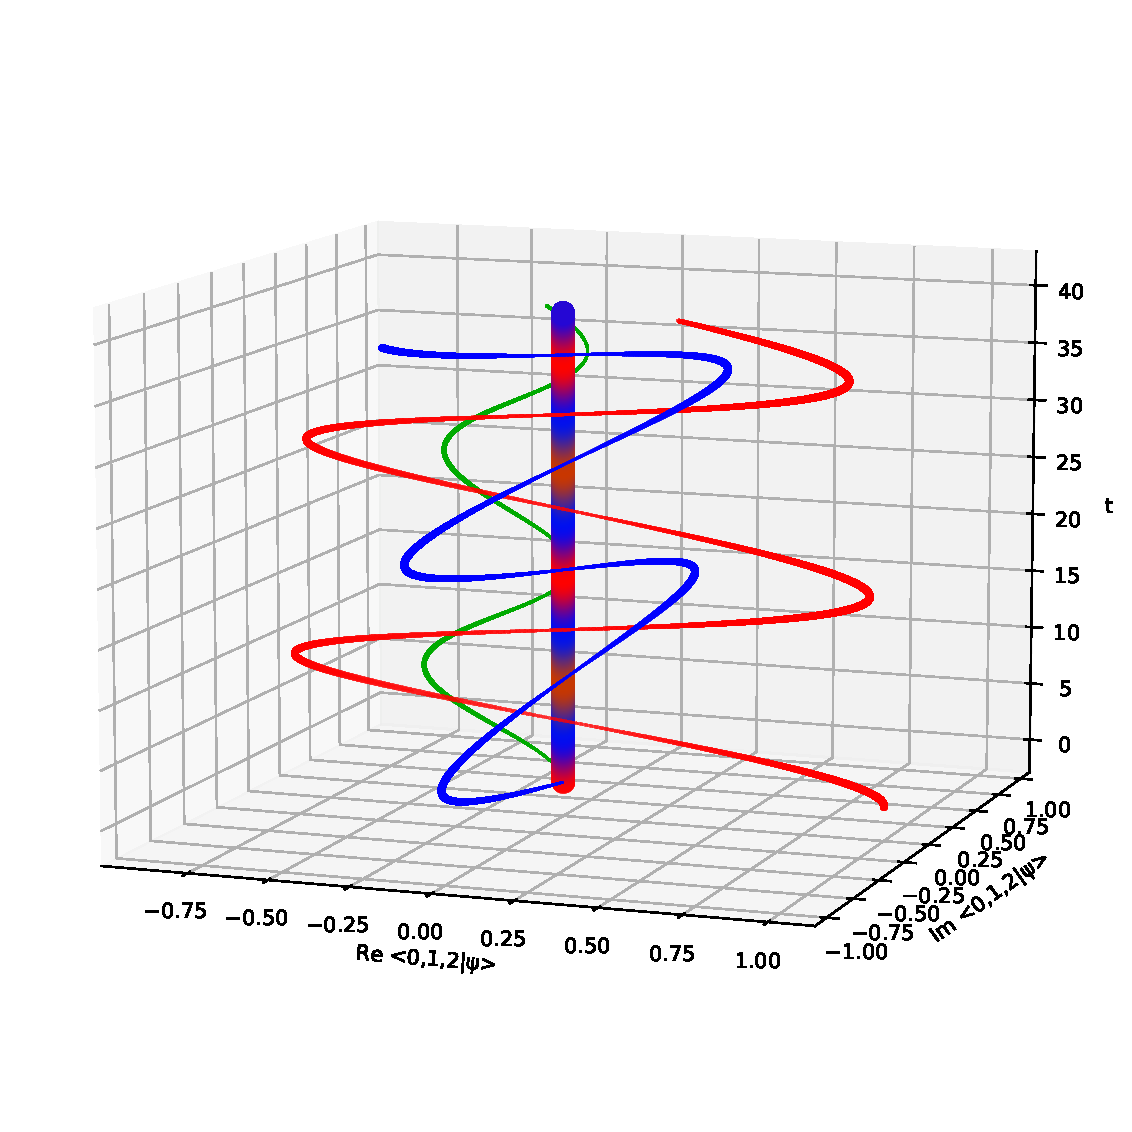
\includegraphics[height=0.45\textheight,clip,trim=80 180 40 140]{img/3ldetect/hermitianSpaceTime_side.pdf}
    \caption{``Side'' view.}
  \end{subfigure}
  \par\bigskip
  \begin{subfigure}[b]{\textwidth}
    \centering
    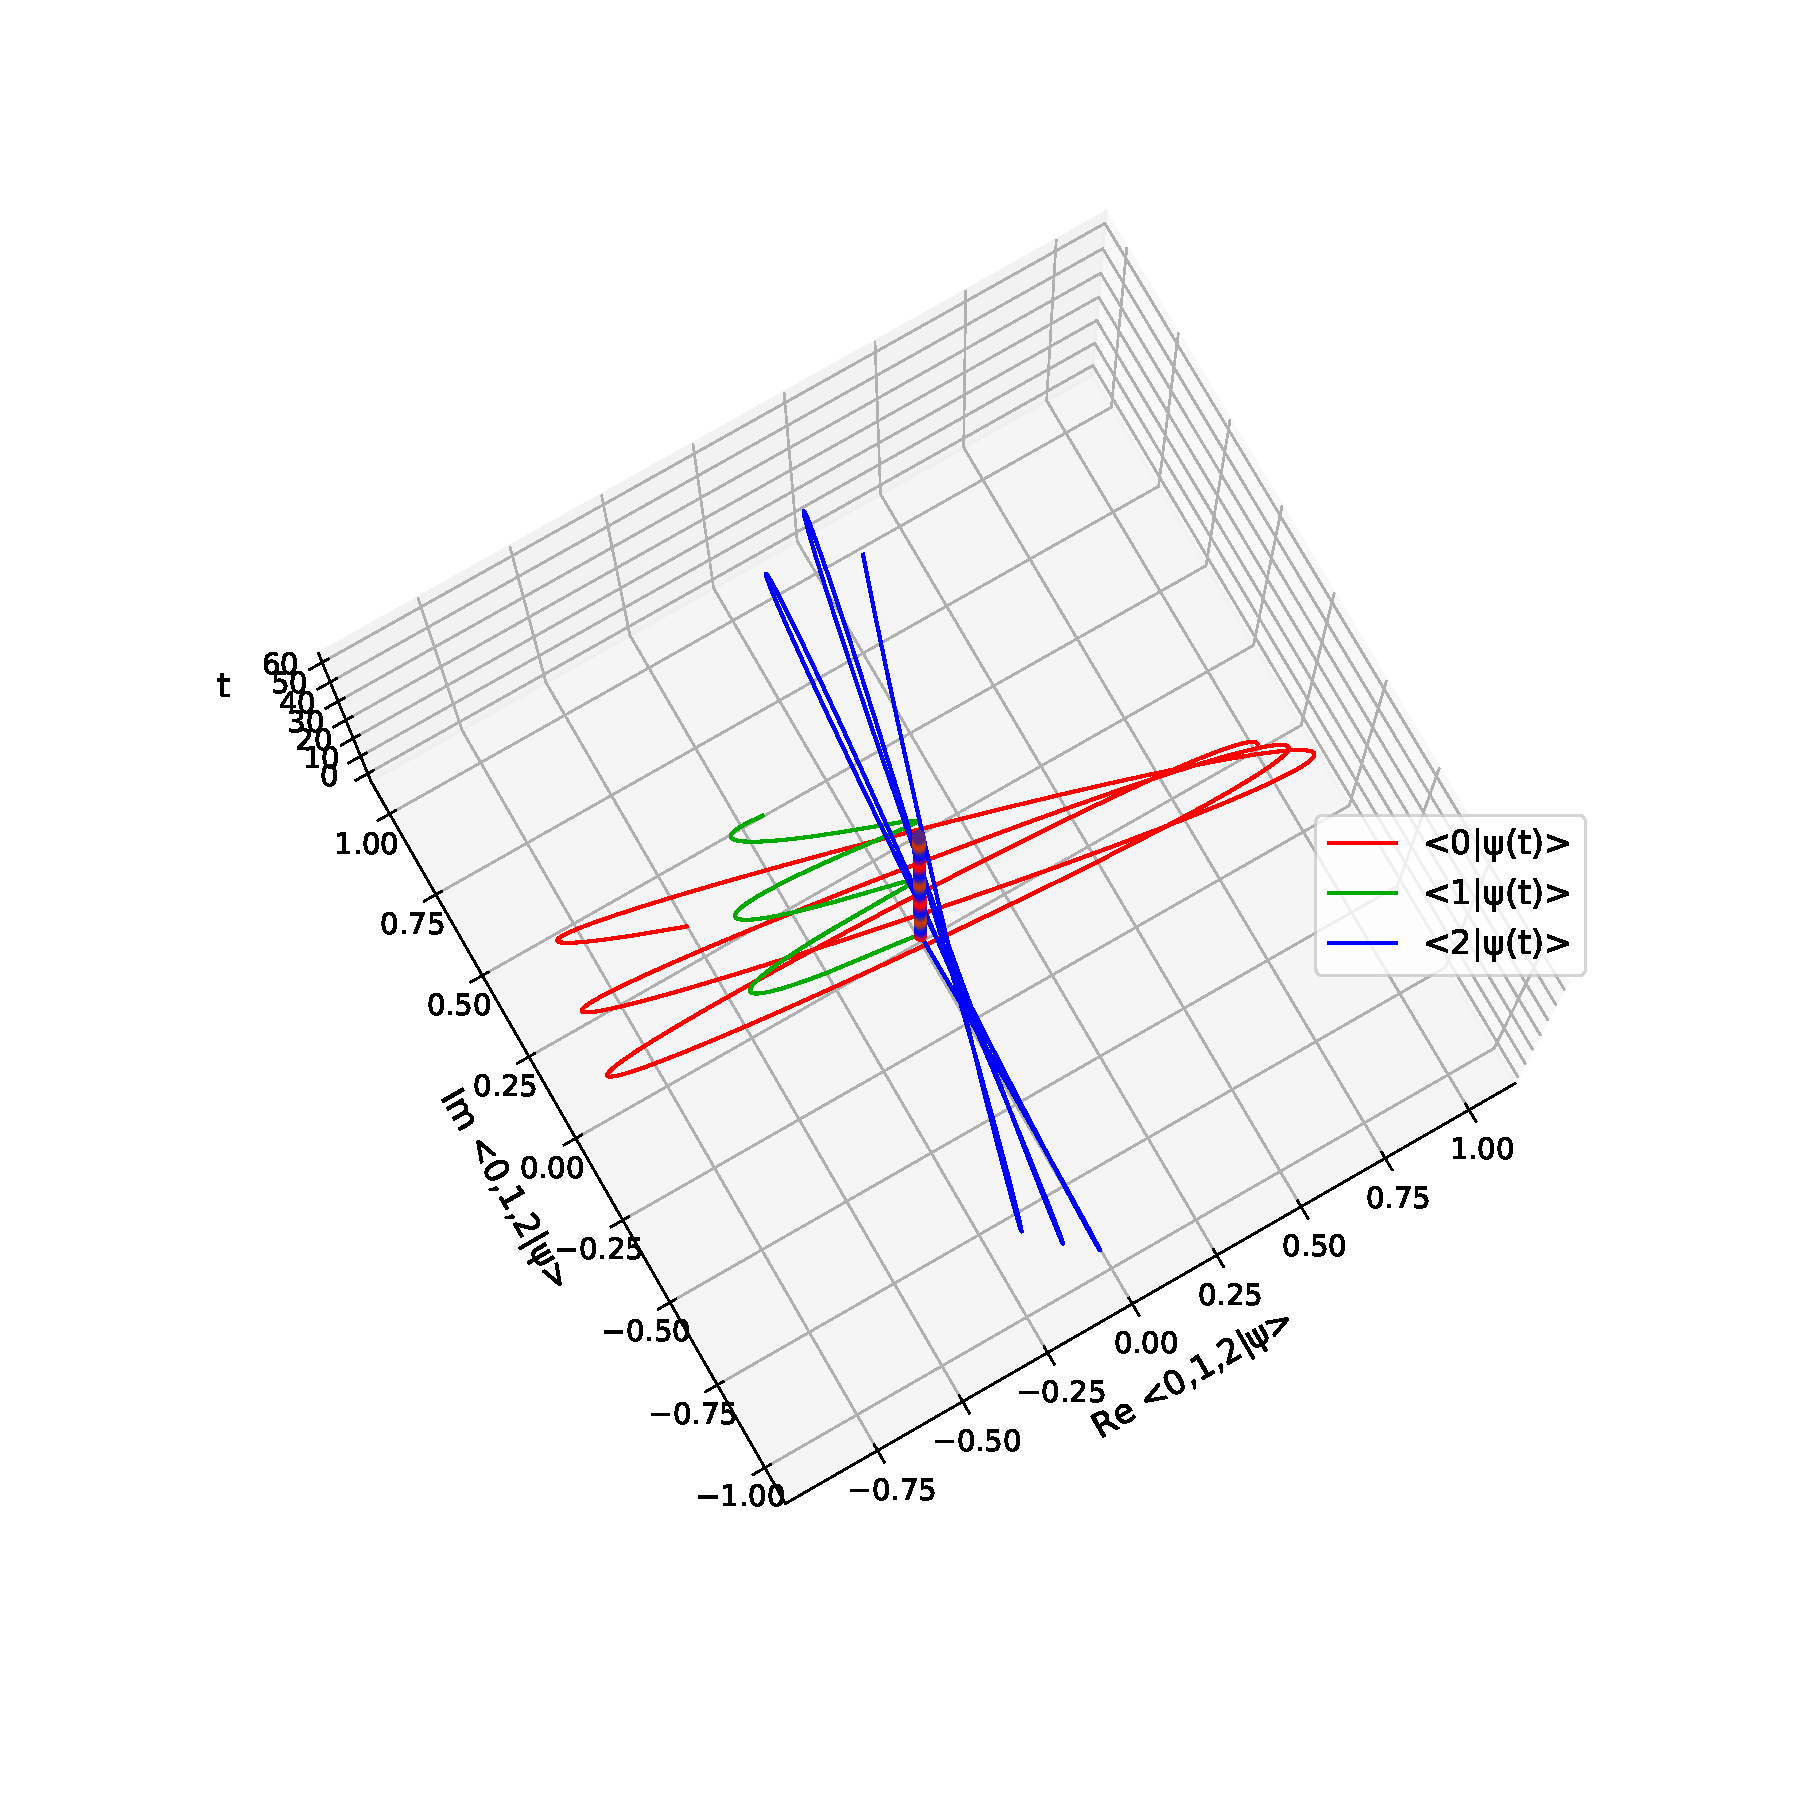
\includegraphics[height=0.41\textheight,clip,trim= 20 120 20 220]{img/3ldetect/hermitianSpaceTime_top.pdf}
    \caption{``Top'' view.}
  \end{subfigure}
  \caption[
    Complex values of the
    probability \emph{amplitudes} $\braket{0, 1, 2}{\psi(t)}$.
  ]{
    \textit{3-D plot} showing the complex values of the
    probability \emph{amplitudes} $\braket{0, 1, 2}{\psi(t)}$.
    Real and imaginary parts of those values are represented on
    the first two axes, while the independent variable (time, $t$)
    is represented
    on the third axis.
    -- Additionally, the vertical axis is coloured to encode \emph{probabilities}
    (absolute values)
    in a similar fashion to Fig. \ref{fig:3lev:probs:lines}. 
  }
  \label{fig:3lev:hermitianEvol}
\end{figure}

\subsection*{\textit{A note on graphical representation}}

Other than visualizing complex-valued functions with three-dimensional plots,
another visualization technique, utilized in various plots in this Section,
consists of leveraging
the fact that the system has exactly 3 levels,
thus allowing three primary colors, red, green and blue, to be combined
in proportion to the probabilities $\abs{\braket{i}{\psi(t)}}$
respectively for $i = 0, 1, 2$. This allows an immediate visualization
of which level, $\ket{0}$, $\ket{2}$ or $\ket{2}$, predominates statistically, if any.
To better clarify this with an example,
a snippet of the implementation of Fig. \ref{fig:3lev:probs} follows.
\begin{lstlisting}[language=Python]
# [...]
import matplotlib
import matplotlib.pyplot as plt

# [...]
for i in 0, 1, 2:
  probs[i] = np.fromiter((prob(t)[i] for t in times), np.float)

# [...]
rgbs = []
for i in range(NPLOTPOINTS):
    rgbs.append(
        (
            probs[0][i],
            probs[1][i],
            probs[2][i]
        )
    )

# [...]
fig, ax = plt.subplots(figsize=(12,6))
ax.set_xlabel('t')
ax.scatter(times, np.zeros(NPLOTPOINTS)-0.1, c=rgbs, marker='|', s=400)
\end{lstlisting}


\subsection{Complex potential -- non-Hermitian evolution}\label{sec:3lev:complexPotential}

In a similar fashion to what seen in Section \ref{sec:hist:detect},
the Hermitian Hamiltonian $\op{H}$, from Eq.~\eqref{eq:3lev:H},
is replaced by
\begin{equation}\label{eq:3lev:nonUnitaryH}
  K \eqbydef \op{H} - \iu \op{D} \text{,}
\end{equation}
where
\begin{equation}\label{eq:3lev:nonUnitaryH:antiHermitianTerm}
  \op{D} \repr \mqty(
    0 &0 &0 \\
    0 &0 &0 \\
    0 &0 &\gamma
  ) \text{.}
\end{equation}
This models the absorptive detection of the ``arrival'' of the system at state~$\ket{2}$.
A numeric value of $\gamma = \mathtt{0.1}$ is chosen for the current simulation.
Repeating the calculation for the time-evolution
brings to
probabilities, and probability amplitudes,
that are graphically visualized in Fig. \ref{fig:3lev:loss3color}, and \ref{fig:3lev:nonHermitianEvol},
and can be compared with the Hermitian (i.e. unitary) case,
Figs. \ref{fig:3lev:probs:stack} and \ref{fig:3lev:hermitianEvol} respectively.
It appears clearly, in Fig. \ref{fig:3lev:loss3color},
that the norm of the state vector is not
conserved, but decreases monotonically. 
%
\begin{figure}[]
  \begin{subfigure}[b]{\textwidth}
    \centering
    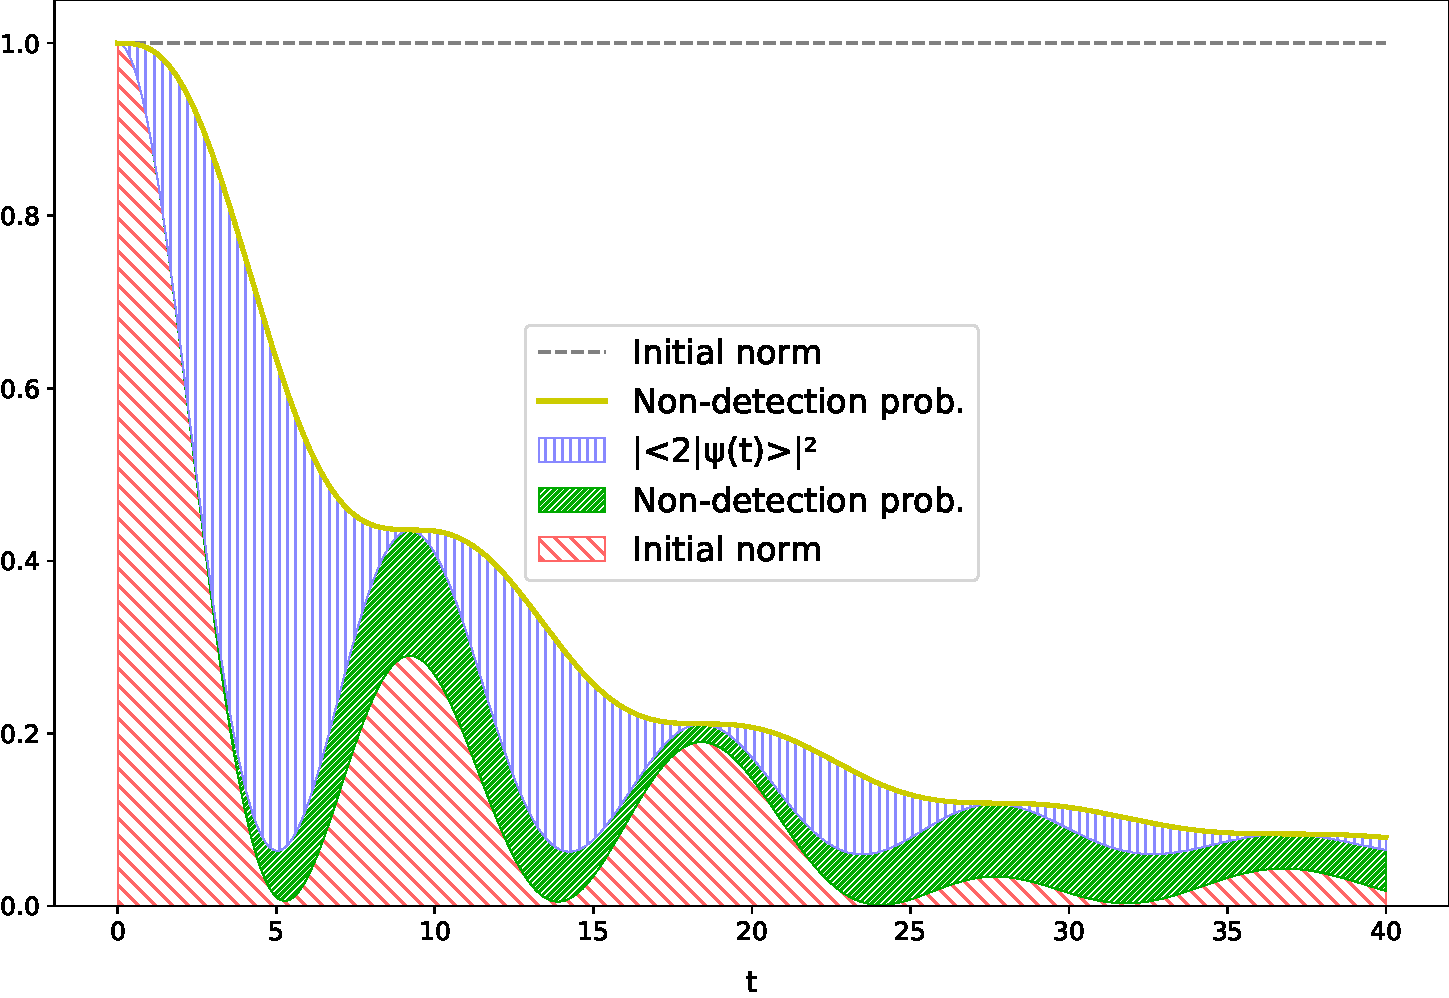
\includegraphics[width=.8\textwidth]{img/3ldetect/loss3color.pdf}
    \subcaption{\setstretch{1.33}
      \emph{Stacked} probability chart (non-Hermitian case) shows that norm
      $\norm{\psi(t)}^2 = \sum_{i=0}^{2} \abs{\braket{i}{\psi(t)}}^2$
      is monotonically decreasing. The actual state probabilities
      will need to be renormalized due to the norm loss of $\ket{\psi(t)}$.
    }
    \label{fig:3lev:loss3color}
  \end{subfigure}
  \par\bigskip
  \par\bigskip
  \begin{subfigure}[b]{\textwidth}
    \centering
    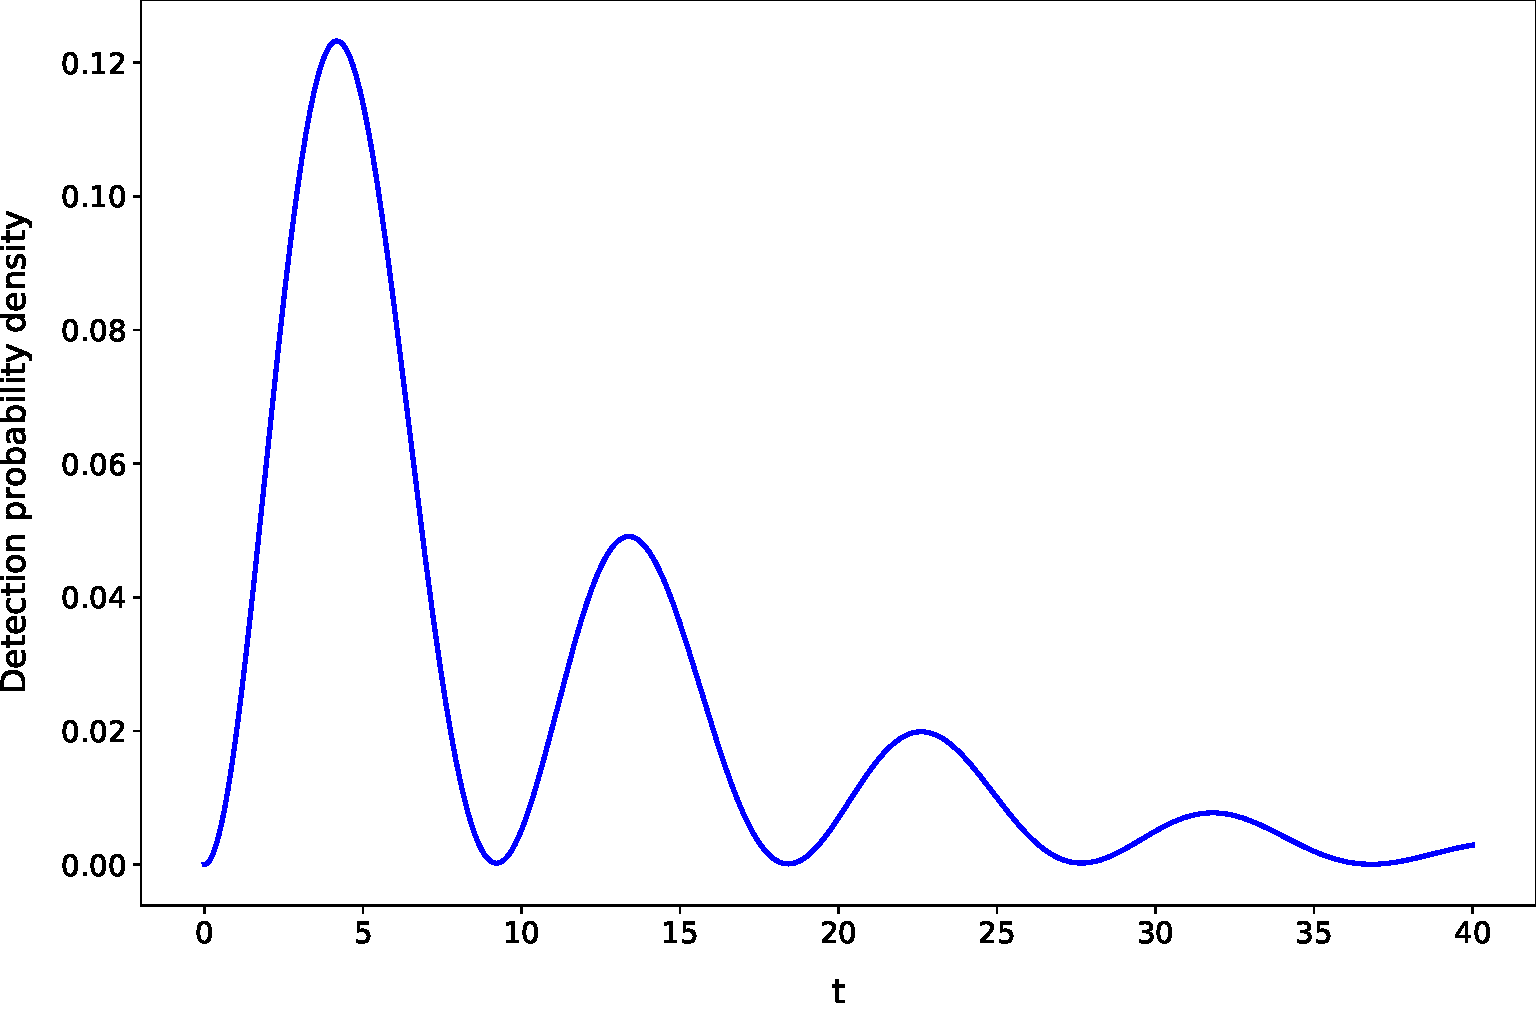
\includegraphics[width=.8\textwidth]{img/3ldetect/loss.pdf}
    \subcaption{
      Normalization loss rate $-\dv{\norm{\psi}^2}{t}$.
      Equates the time-of-arrival probability distribution (at the ``absorbing'' state $\ket{2}$).
    }
    \label{fig:3lev:loss}
  \end{subfigure}
  \par\bigskip
  \par\bigskip
  \caption{
    Absorptive detector model: norm loss and probabilities.
  }
  \label{fig:3lev:nonHermitianProbs}
\end{figure}
%
\begin{figure}[]
  \begin{subfigure}[b]{\textwidth}
    \centering
    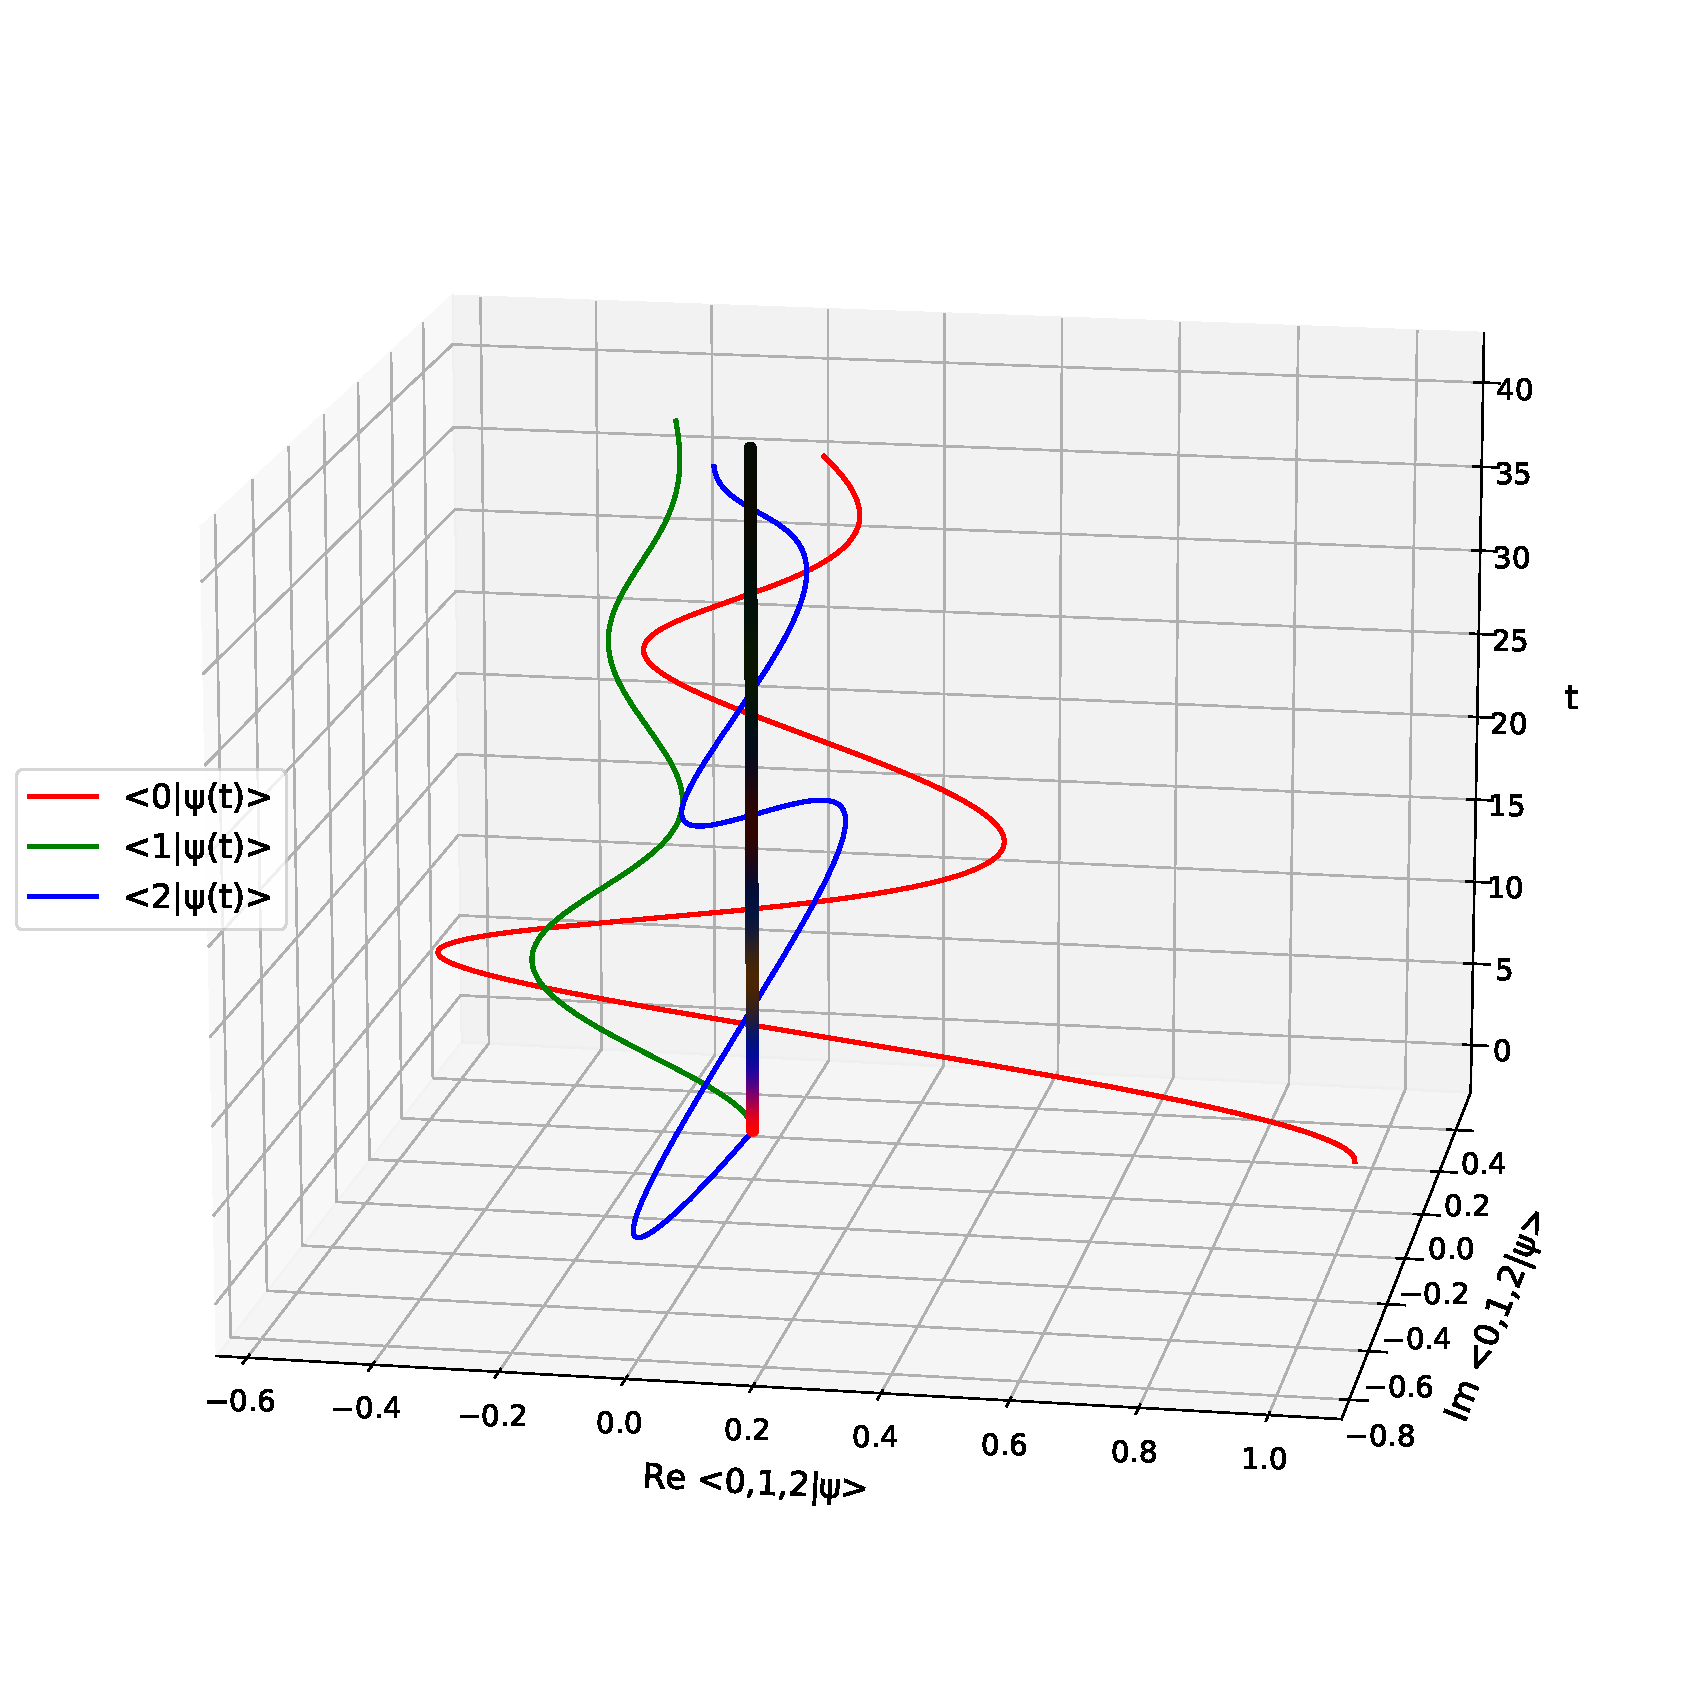
\includegraphics[height=0.41\textheight,clip,trim=0 90 40 140]{img/3ldetect/NonHermitianSpaceTime_side.pdf}
    \caption{``Side'' view.}
  \end{subfigure}
  \par\bigskip
  \begin{subfigure}[b]{\textwidth}
    \centering
    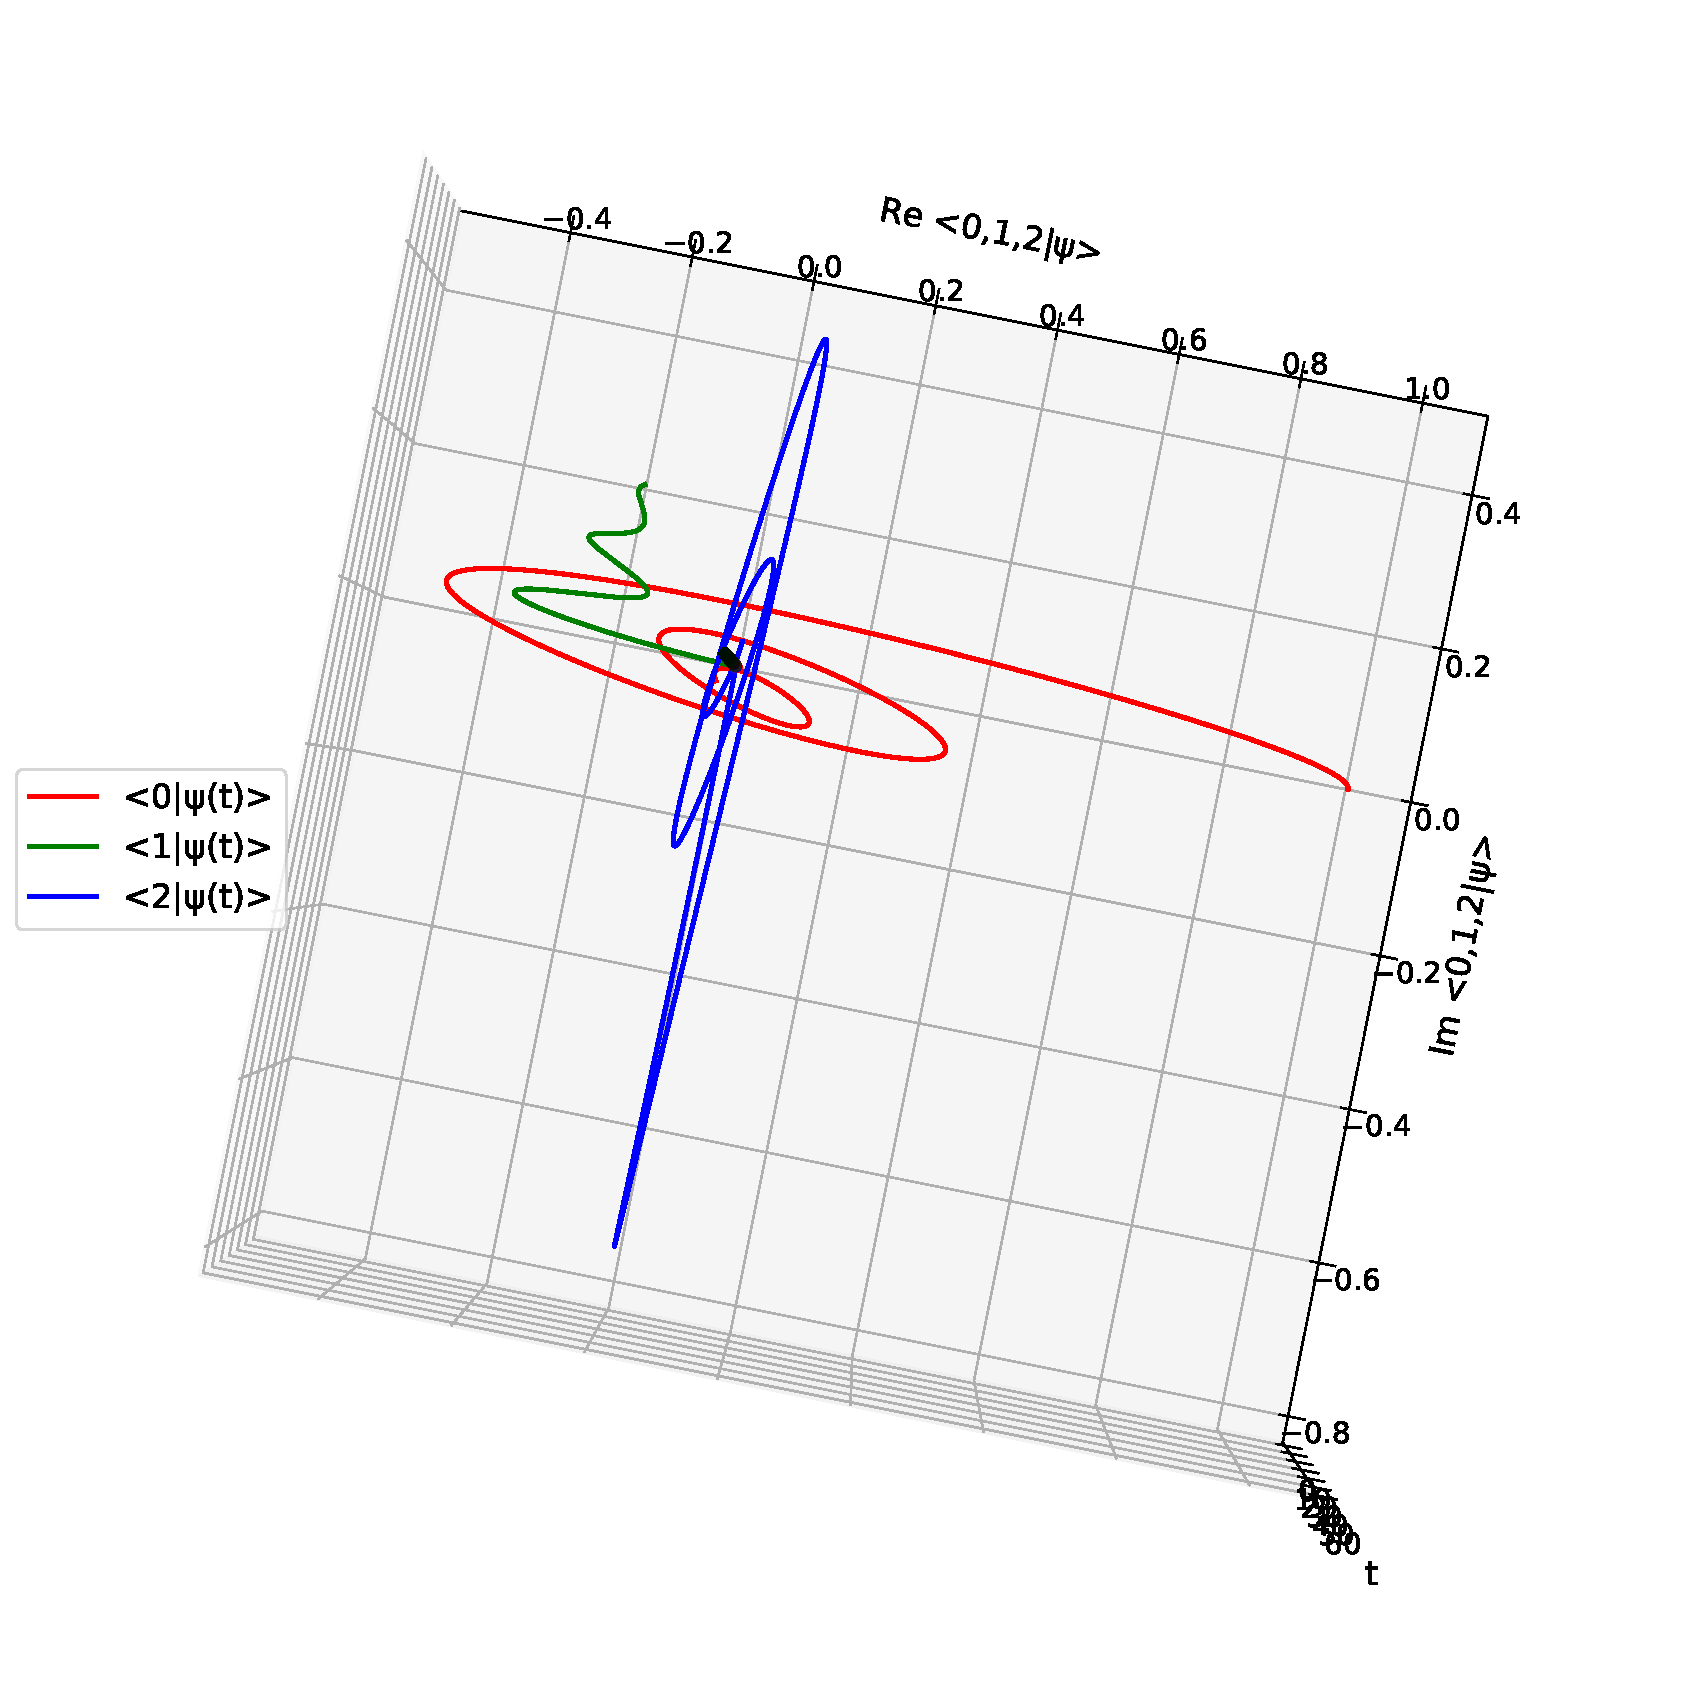
\includegraphics[height=0.44\textheight,clip,trim= 0 90 20 75]{img/3ldetect/NonHermitianSpaceTime_top.pdf}
    \caption{``Top'' view.}
  \end{subfigure}
  \caption[
    Probability amplitudes, with ``lossy'' norm
  ]{
    Non-Hermitian evolution: 3-D complex plot: probability amplitudes, with ``lossy''
    norm (visually, lines get closer to the time axis as $t$ increases).
  }
  \label{fig:3lev:nonHermitianEvol}
\end{figure}

According to the absorptive detector model, the loss of normalization
$-\dv{\norm{\psi}^2}{t}$ indicates the probability of detection
with respect to time, in other words: the time-of-arrival
probability distribution. It is plotted in Fig. \ref{fig:3lev:loss}.

The same results
about probabilities and normalization loss
are plotted
over a longer time interval
in Fig.~\ref{fig:3lev:nonHermitianProbs_ext}.
By comparing the latter,
back with Fig.~\ref{fig:3lev:probs:stack},
it's apparent that in the unitary case the system
periodically oscillates between $\ket{0}$ and $\ket{2}$
---transitioning through the intermediate level $\ket{1}$,
but with a small value of $\abs{\braket{1}{\psi(t)}}^2$.
Instead, within the non-unitary evolution, and with the chosen parameters,
the system is ``driven'' from $\ket{0}$ to $\ket{1}$ and,
after a transient oscillation between the three levels,
shows an asymptotic behavior.
The fidelity with respect to $\ket{1}$,
$\frac{\abs{\braket{1}{\psi(t)}}^2}{\norm{\psi(t)}^2}$,
evaluated numerically at $t=150$ is given by
\begin{lstlisting}[language=Python]
# Pick the last value of time
times_extended[-1]
\end{lstlisting}
\begin{lstlisting}
150.0
\end{lstlisting}
\begin{lstlisting}[language=Python]
# Fidelity
(np.abs(evolution_extended[1])**2)[-1] / norms_extended[-1]**2
\end{lstlisting}
The result is about $94\%$.
\begin{lstlisting}
0.9414855990054901
\end{lstlisting}
It's also worth noting that the norm does not fully vanish with $t \rightarrow +\infty$,
meaning there is a finite probability that detection (or ``absorption'', or spontaneous decay) never happens:
\begin{equation*}
  P_{\mathrm{nd}} = \lim_{t \rightarrow +\infty} 1 - \norm{\psi(t)}^2 \text{.}
\end{equation*}
At the ``large'' value of $t=150$ of our numerical computation, this yields
\begin{lstlisting}[language=Python]
norms_extended[-1]**2
\end{lstlisting}
\begin{lstlisting}
0.05684539507975811
\end{lstlisting}
i.e. roughly 6\% of non-absorption probability.
%
\begin{figure}[]
  \begin{subfigure}[b]{\textwidth}
    \centering
    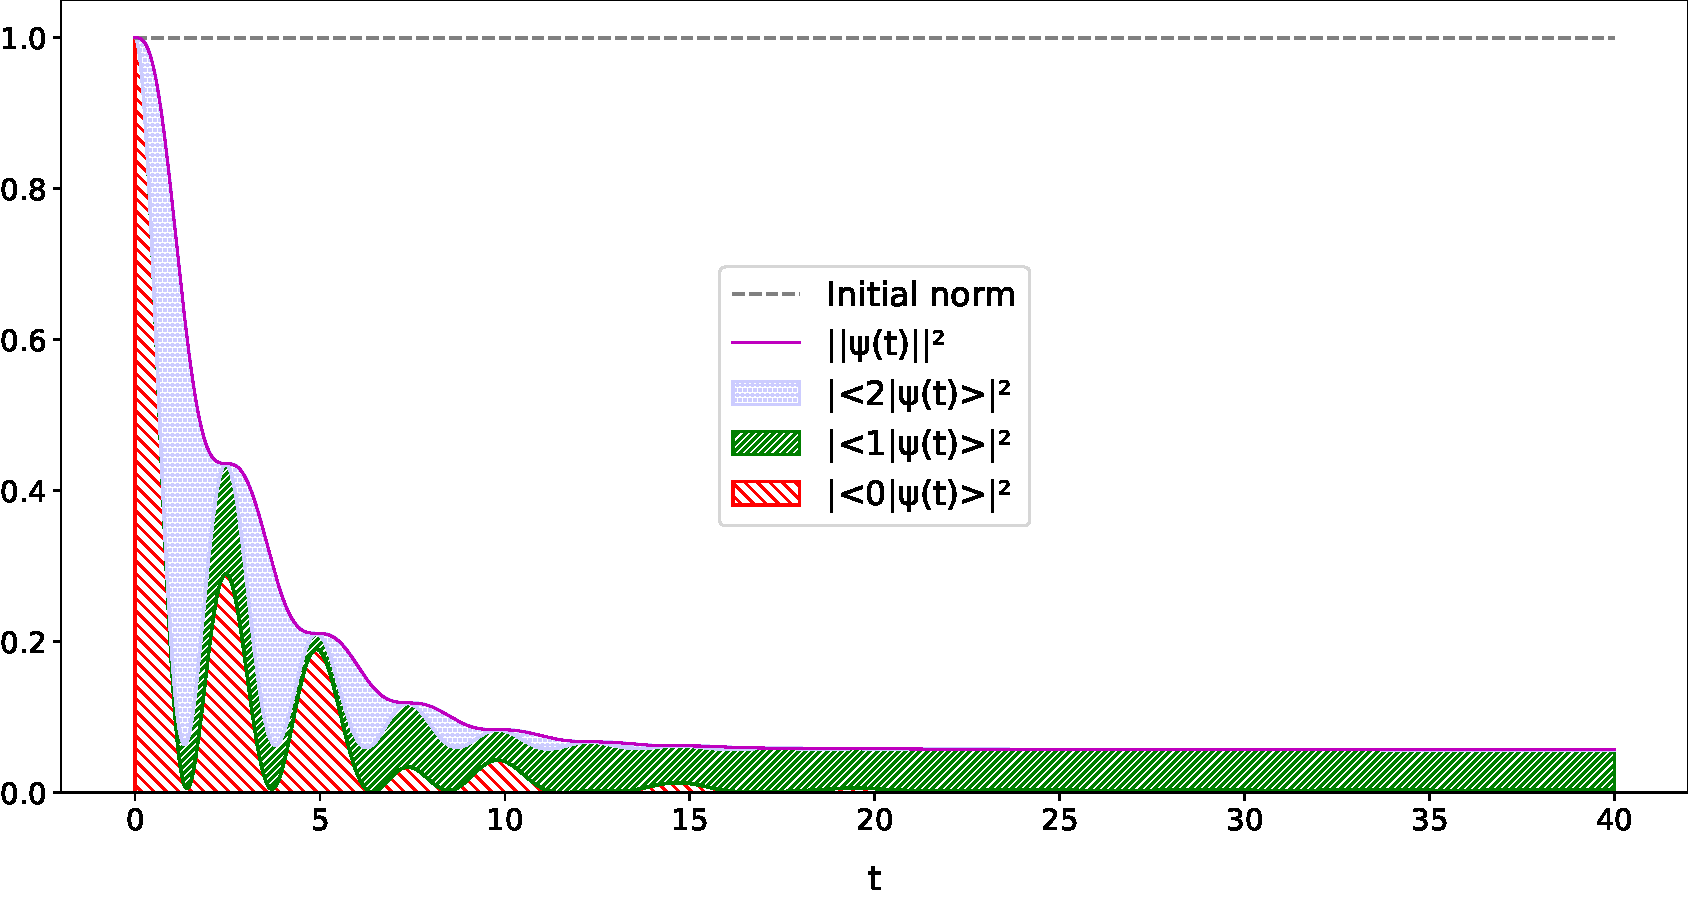
\includegraphics[width=\textwidth]{img/3ldetect/loss3color_ext.pdf}
    \subcaption{
      Probabilities and normalization loss.
    }
    \label{fig:3lev:loss3color_ext}
  \end{subfigure}
  \par\bigskip
  \par\bigskip
  \begin{subfigure}[b]{\textwidth}
    \centering
    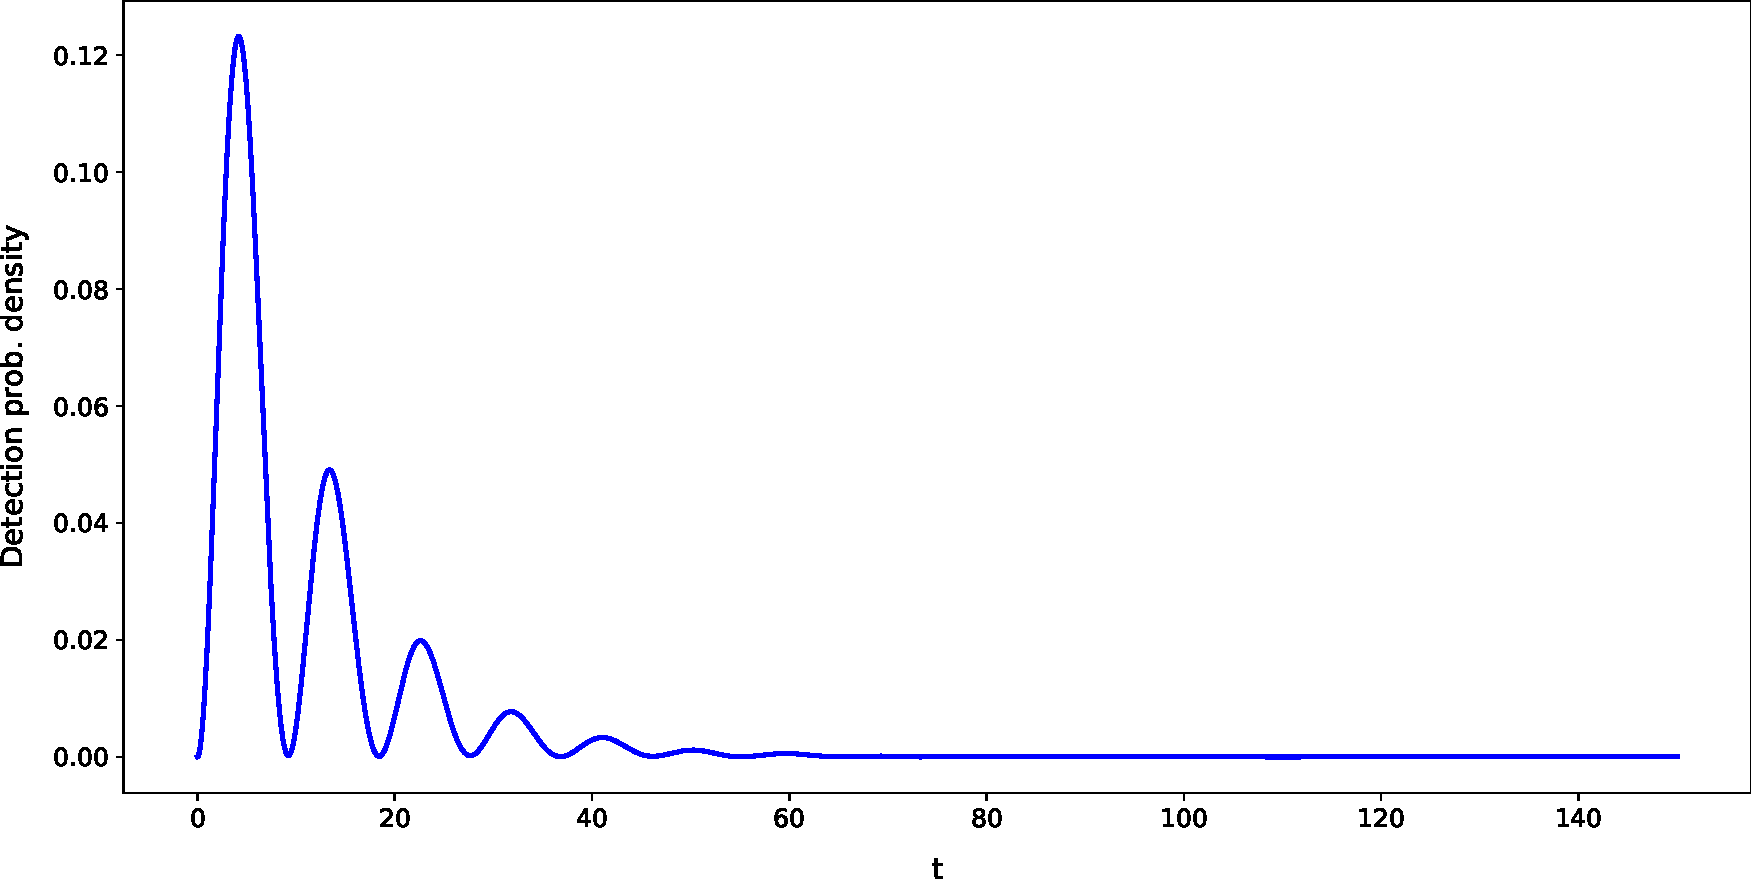
\includegraphics[width=\textwidth]{img/3ldetect/loss_ext.pdf}
    \subcaption{
      Normalization loss rate, or time-of-arrival probability distribution.
    }
    \label{fig:3lev:loss_ext}
  \end{subfigure}
  \par\bigskip
  \par\bigskip
  \caption[
    Absorptive detector model: evolution over a longer time interval.
  ]{
    Absorptive detector model: same results as in Fig.~\ref{fig:3lev:nonHermitianProbs},
    over a longer time interval.
  }
  \label{fig:3lev:nonHermitianProbs_ext}
\end{figure}

\subsection{Discrete Page--Wootters}

Let us consider a Page--Wootters \emph{discrete} clock, with $N_{T}$ levels,
i.e. the clock Hilbert space has finite dimension $N_{T}$,
where we choose $N_{T} = 60$
(somehow resembling the 60 ticks indicating minutes or seconds
in a conventional clock\footnote{
  For an intuitive, and suggestive, depiction, the reader may want to look at \cite[Fig.~1]{QClockPic},
  where the quantum levels of the clock are $N_{T} = 12$
  ---please note, however, that the paper allows for the clock
  and the remaining system to \emph{interact}, whereas, in the original formulation
  of the Page--Wootters mechanism,
  they are only \emph{entangled}.
}).

Let also $N_S$ indicate the Hilbert space dimension of the of ``the rest of the universe'' $\hilb{H}_S$
(in the sense of \cite{Marletto:Evolution}, among others). In the current example
it is $N_S = 3$.

A basis of $\hilb{H}_T$ is chosen where the time operator $\op{T}$ is diagonal:
\begin{equation}
  \op{T} \repr \frac{\Delta T}{N_T} \mqty(
                                          0       &0      &\ldots &0        \\
                                          0       &1      &\ldots &0        \\
                                          \vdots  &\vdots &\ddots &\vdots   \\
                                          0       &0      &\ldots &N_{T}-1
                                        ) \text{,}
\end{equation}
where $\Delta T$ if the time interval under study.
And the frequency operator $\op{\Omega}$ is computed via \term{Discrete Fourier Transform (DFT)}:
\begin{equation}
  \op{\Omega} = \frac{2\pi N_T}{\Delta{T}^2} F^{\dagger} \op{T} F \text{.}
\end{equation}
It's worth noting that, from a numerical computation perspective,
different library implementations use different conventions and definitions
for the discrete Fourier matrix. Therefore,
appropriate factors in the relation between $\op{T}$ and $\op{\Omega}$
may be required.
In our code:
\begin{lstlisting}[language=Python]
# [...]
TMIN, TMAX = 0, 40
TMIN_N, TMAX_N = float(TMIN), float(TMAX)

# [...]
from scipy.linalg import dft, norm, expm, det, inv

# [...]
# Number of levels of the clock aka dimension of Time Hilbert space
NT = 60

# Time interval under study
DT = TMAX_N  # assume we start with time 0

# Time operator
T = DT * np.diag(np.arange(NT)) / NT

# Discrete Fourier
F = dft(NT, scale='sqrtn')
F_dagger = F.conj().T

# Frequency operator
Omega = F_dagger @ T @ F * 2*np.pi * NT / DT**2
\end{lstlisting}

Then the ``Hamiltonian'' ${\mathbb{J}}$, acting on $\pwspace$, and defined in Eq.~\eqref{eq:pwHamiltonian:nonUnitary}
is derived, with eigenvalues and eigenvectors::
\begin{lstlisting}[language=Python]
J = np.kron(Omega, np.eye(3)) + np.kron(np.eye(NT), K())
 
eigenvalues, eigenvectors = np.linalg.eig(J)
eigenvectors = eigenvectors.T
\end{lstlisting}
where the Python function \verb|K()| is the non-Hermitian operator $K$ of Eq.~\eqref{eq:3lev:nonUnitaryH}.

Eigenvectors need to be ``initially normalized in $\hilb{H}_S$'' in the sense
of a state vector $\ket{\psi(t)}$ satisfying
$\norm{\psi(0)}^2=1$ or,
 in Page--Wootters terms,
 a vector $\dket{\Psi}$, in $\pwspace$, satisfying
 $\langle\langle \Psi | 0 \rangle_{T}\langle 0 | \Psi \rangle \rangle = 1$.
\begin{lstlisting}[language=Python]
eigenvectors_normalized_in_S = np.empty((NT*NS, NT*NS), dtype=complex)
for i in range(NT*NS):
    eigenvectors_normalized_in_S[i] = eigenvectors[i] / norm(eigenvectors[i][:3])
\end{lstlisting}

A ``phase correction'' may be needed in order to allow a comparison with
the time evolution predicted with ``standard'' quantum mechanics
(although, still, with a non-Hermitian Hamiltonian, or \emph{complex potential}).
Namely,
corrections related to non-zero eigenvalues are required ---see Eq.~\eqref{eq:pw:non0e:last}.
It's worth recalling that,
as the Wheeler-DeWitt equation reads $\mathbb{J} \dket{\Psi} = 0$,
eigenvectors of $\mathbb{J}$ related to eigenvalues ---say, $\epsilon_{i}$---
which are not zero,
need to be corrected by ``rigidly shifting the spectrum of $H_{S}$
by [$\epsilon_{i}$]'' (once again, \cite[``\textit{The Zero-eigenvalue}'']{Lloyd:Time}):
\begin{equation}
  \dket{\epsilon_i} \;\longrightarrow\; \dket{\Phi_{i}} \eqbydef e^{ -\iu \op{T} \epsilon_{i} \, \ox \, \idop_{S}} \dket{\epsilon_{i}} \text{,}
  \label{eq:3lev:correction}
\end{equation}
where it has been set $\hbar=1$. This translates in code as follows:\footnote{
  In the Python code, \Verb+i+ is an iteration index and \Verb|1j| is the imaginary unit
  (the latter is a convention of the language).
  In eq.\eqref{eq:3lev:correction},
  $i$ is a summation index and $\iu$ (upright typeface) is the imaginary unit.
  The context may also help in interpreting the notation correctly.
}
\begin{lstlisting}[language=Python]
histories = np.empty((NT*NS, NT*NS), dtype=complex)

for i in range(NT*NS):
    histories[i] = \
        expm(np.kron( -1j*T*eigenvalues[i], np.eye(NS) )) @ \
        eigenvectors_normalized_in_S[i]
\end{lstlisting}
%
With a slightly different notation,
the \Verb|histories[i]|
correspond to the $\dket{\Phi_i}$ in Eq.~\eqref{eq:3lev:correction}.
They are named \Verb!histories! because each of them
(and any linear combination, per quantum superposition principle)
encodes a possible evolution (although with discrete time resolution)
of the system along the whole time interval $[0, \Delta T]$.

A comparison can be made, in principle, between the quantities
\begin{align}\begin{split}\label{eq:3lev:PWComparison}
  \bradket{t_n}{\Psi} \sim  &\ket{\psi(t_n)},\\
                            &\forall n = 0, \dots, N_{T}-1
\end{split}\end{align}
where \[ t_{n} = \frac{n\Delta T}{N_T} \]
and
$\dket{\Psi}$ is one of the ${\dket{\Phi_{i=0,\dots,N_T N_S - 1}}}$,
or a linear combination of them,
so that
\begin{equation}\label{eq:3lev:PWInitialCond}
  \prescript{}{T}{\bradket{0}{\Psi}} = \ket{\psi_0}_S \text{.}
\end{equation}

\subsubsection*{Initial value problem}

As there isn't an individual $\dket{\Phi_i}$,
in our numeric example,
satisfying the \eqref{eq:3lev:PWInitialCond},
a suitable linear combination
$\dket{\Psi} \eqbydef \sum_{i=0}^{N_{T}N_{S}-1} c_{i}\dket{\Phi_i}$
needs to be found. Algebraically, the problem consists in
$N_{S}$ linear equations
in $N_{T}N_{S}$ variables, therefore there is certainly more than one solution
---a solution space of dimension $(N_{T} - 1)N_{S}$ indeed.

The following algorithm, among infinite possibilities,
and merely for reasons of numerical stability,
picks $N_S$
vectors, say,
\[
  \dket{\Phi_i}, \dket{\Phi_j}, \dket{\Phi_k}
\]
(for $N_S = 3$),
so that, \emph{to the best approximation},
\[
  \prescript{}{T}{\bradket{0}{\Phi_i}}, \;
  \prescript{}{T}{\bradket{0}{\Phi_j}}, \;
  \prescript{}{T}{\bradket{0}{\Phi_k}}
\]
form an orthonormal basis in $\hilb{H}_S$.%
\footnote{
  ``Best approximation'' (of an orthonormal base in $\hilb{H}_S$)
  in the sense of finding
  three (or in general $N_S$) different
  $i, j, k \in \{0, \dots, N_{S}-1\}$ that minimize
  $
    \abs{1 - \det\mqty(
      & \prescript{}{S}{\bra{0}}   \prescript{}{T}{\bradket{0}{\Phi_i}}
      & \prescript{}{S}{\bra{1}}   \prescript{}{T}{\bradket{0}{\Phi_i}}
      & \prescript{}{S}{\bra{2}}   \prescript{}{T}{\bradket{0}{\Phi_i}}
      \\
      & \prescript{}{S}{\bra{0}}   \prescript{}{T}{\bradket{0}{\Phi_j}}
      & \prescript{}{S}{\bra{1}}   \prescript{}{T}{\bradket{0}{\Phi_j}}
      & \prescript{}{S}{\bra{2}}   \prescript{}{T}{\bradket{0}{\Phi_j}}
      \\
      & \prescript{}{S}{\bra{0}}   \prescript{}{T}{\bradket{0}{\Phi_k}}
      & \prescript{}{S}{\bra{1}}   \prescript{}{T}{\bradket{0}{\Phi_k}}
      & \prescript{}{S}{\bra{2}}   \prescript{}{T}{\bradket{0}{\Phi_k}}
    )}
  $.
}
Then it's elementary linear algebra to find out the $N_S$
coefficients
% \footnote{
%   $N_S$ coefficients (3 in our example),
%   instead of $N_S N_T$ (180 in our example)
%   as the dimension of $\pwspace$ would otherwise suggest.
%   This is because the condition is only on $\prescript{}{T}{\bradket{0}{\Psi}}$
%   and not on the ``entire'' $\dket{\Psi}$.
% }
---say $a$, $b$ and $c$---
so that \begin{equation}\label{eq:3lev:initialLinEq}
  a\cdot\prescript{}{T}{\bradket{0}{\Phi_i}} +
  b\cdot\prescript{}{T}{\bradket{0}{\Phi_j}} +
  c\cdot\prescript{}{T}{\bradket{0}{\Phi_k}} =
  \ket{\psi_0} .
\end{equation}
With these coefficients, it will be
\begin{equation}\label{eq:3lev:PhiLinearComb}
  \dket{\Psi} =
  a\cdot\dket{\Phi_i} +
  b\cdot\dket{\Phi_j} +
  c\cdot\dket{\Phi_k}
\end{equation}
the (Page--Wootters) ``history vector'' to be plugged in \eqref{eq:3lev:PWComparison}
for comparison with standard quantum mechanics.

Full implementation code is available at Appendix
\ref{appendix:jupyter:3lev:page-wootters},
function \\
\Verb#find_linear_independent_initial()#
% \footnote{
%   The current implementation is strongly based on the assumption that $N_S = 3$.
%   From a computing perspective,
%   efficient and scalable support for higher $N_S$
%   would require some \term{refactoring} \parencite{comp:refactor}.
%   However,
%   the aim in this case is merely illustrating the \emph{physics} of this class of systems,
%   providing an effective \term{proof of concept} \parencite{comp:poc}.
% }
returns:
\begin{lstlisting}[language=Python]
def find_linear_independent_initial(eigenvectors=eigenvectors_normalized_in_S):

  # [...]
  return best_i, best_j, best_k, best_det
\end{lstlisting}
Then it's invoked:
\begin{lstlisting}[language=Python]
best_i, best_j, best_k, best_det = find_linear_independent_initial()
\end{lstlisting}
and (the coefficients of) the linear combination is (are) derived.
The following resolves \eqref{eq:3lev:initialLinEq}:
\begin{lstlisting}[language=Python]
states = np.array([
    histories[best_i][:NS],
    histories[best_j][:NS],
    histories[best_k][:NS]
])

# Find what linear combination would bring to the desired initial state psi_0_n
coeffs = inv(states.T) @ psi_0
\end{lstlisting}
and
\begin{lstlisting}[language=Python]
history = coeffs.dot(np.array([
    histories[best_i],
    histories[best_j],
    histories[best_k]
]))
\end{lstlisting}
implements \eqref{eq:3lev:PhiLinearComb}.

\subsubsection*{Comparison}

The following code
(with notation slightly changed compared to Appendix~\ref{appendix:jupyter:3lev:page-wootters}, for clarity)
\begin{lstlisting}[language=Python]
pwpsi = history.reshape((-1,NS)).T
\end{lstlisting}
rearranges the \Verb!history! array in such a way that
\begin{lstlisting}[language=Python]
pwpsi[m][n]
\end{lstlisting}
is
\begin{equation*}
\prescript{}{S}{\bra{m}} \prescript{}{T}{\bradket{t_n}{\Psi}}
\end{equation*}
and can be compared with
\begin{equation*}
  \braket{m}{\psi(t_n)} 
\end{equation*}
from ``ordinary'' quantum mechanics, $
  \forall \; m \in \{0, \dots, N_S - 1\} \text{ and } n \in \{0, \dots, N_T - 1\}
$.

Such comparison is visualized in Fig.~\ref{fig:3lev:PWSpaceTimeFit},
showing excellent agreement between the discrete Page--Wootters model (square points)
and ``standard'' quantum evolution (continuous line).
Page--Wootters ``history vector'' components are also shown on their own
in Fig.~\ref{fig:3lev:PWSpaceTime}. 

\begin{figure}[]
  \begin{subfigure}[b]{\textwidth}
    \centering
    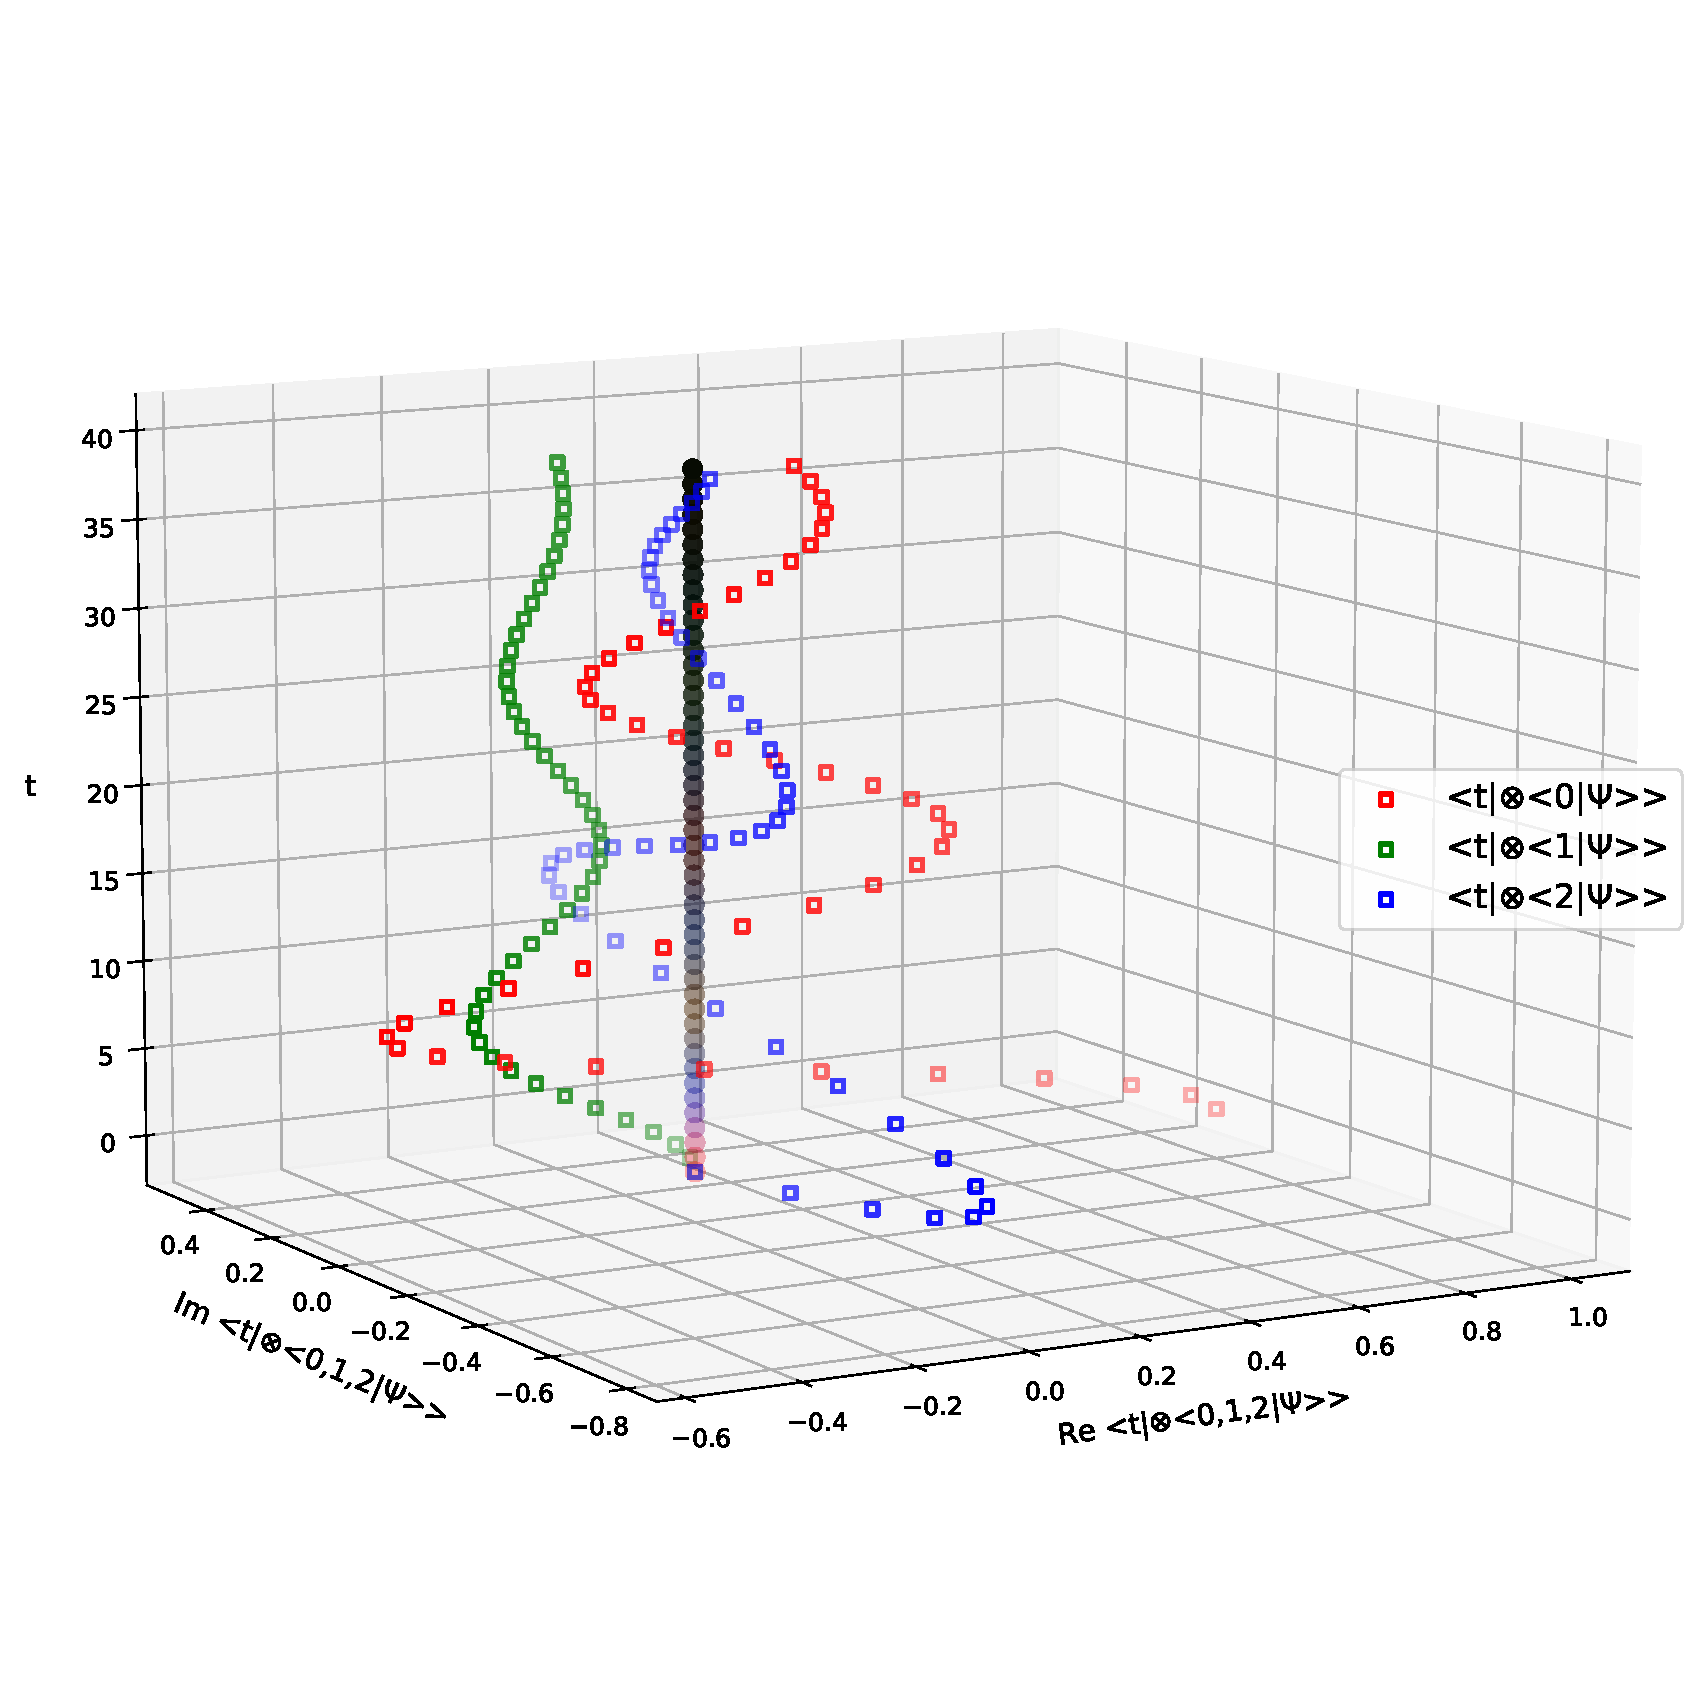
\includegraphics[height=0.41\textheight,clip,trim=0 90 0 140]{img/3ldetect/PWSpaceTime_side.pdf}
    \caption{3-D plot: side view.}
  \end{subfigure}
  \par\bigskip
  \begin{subfigure}[b]{\textwidth}
    \centering
    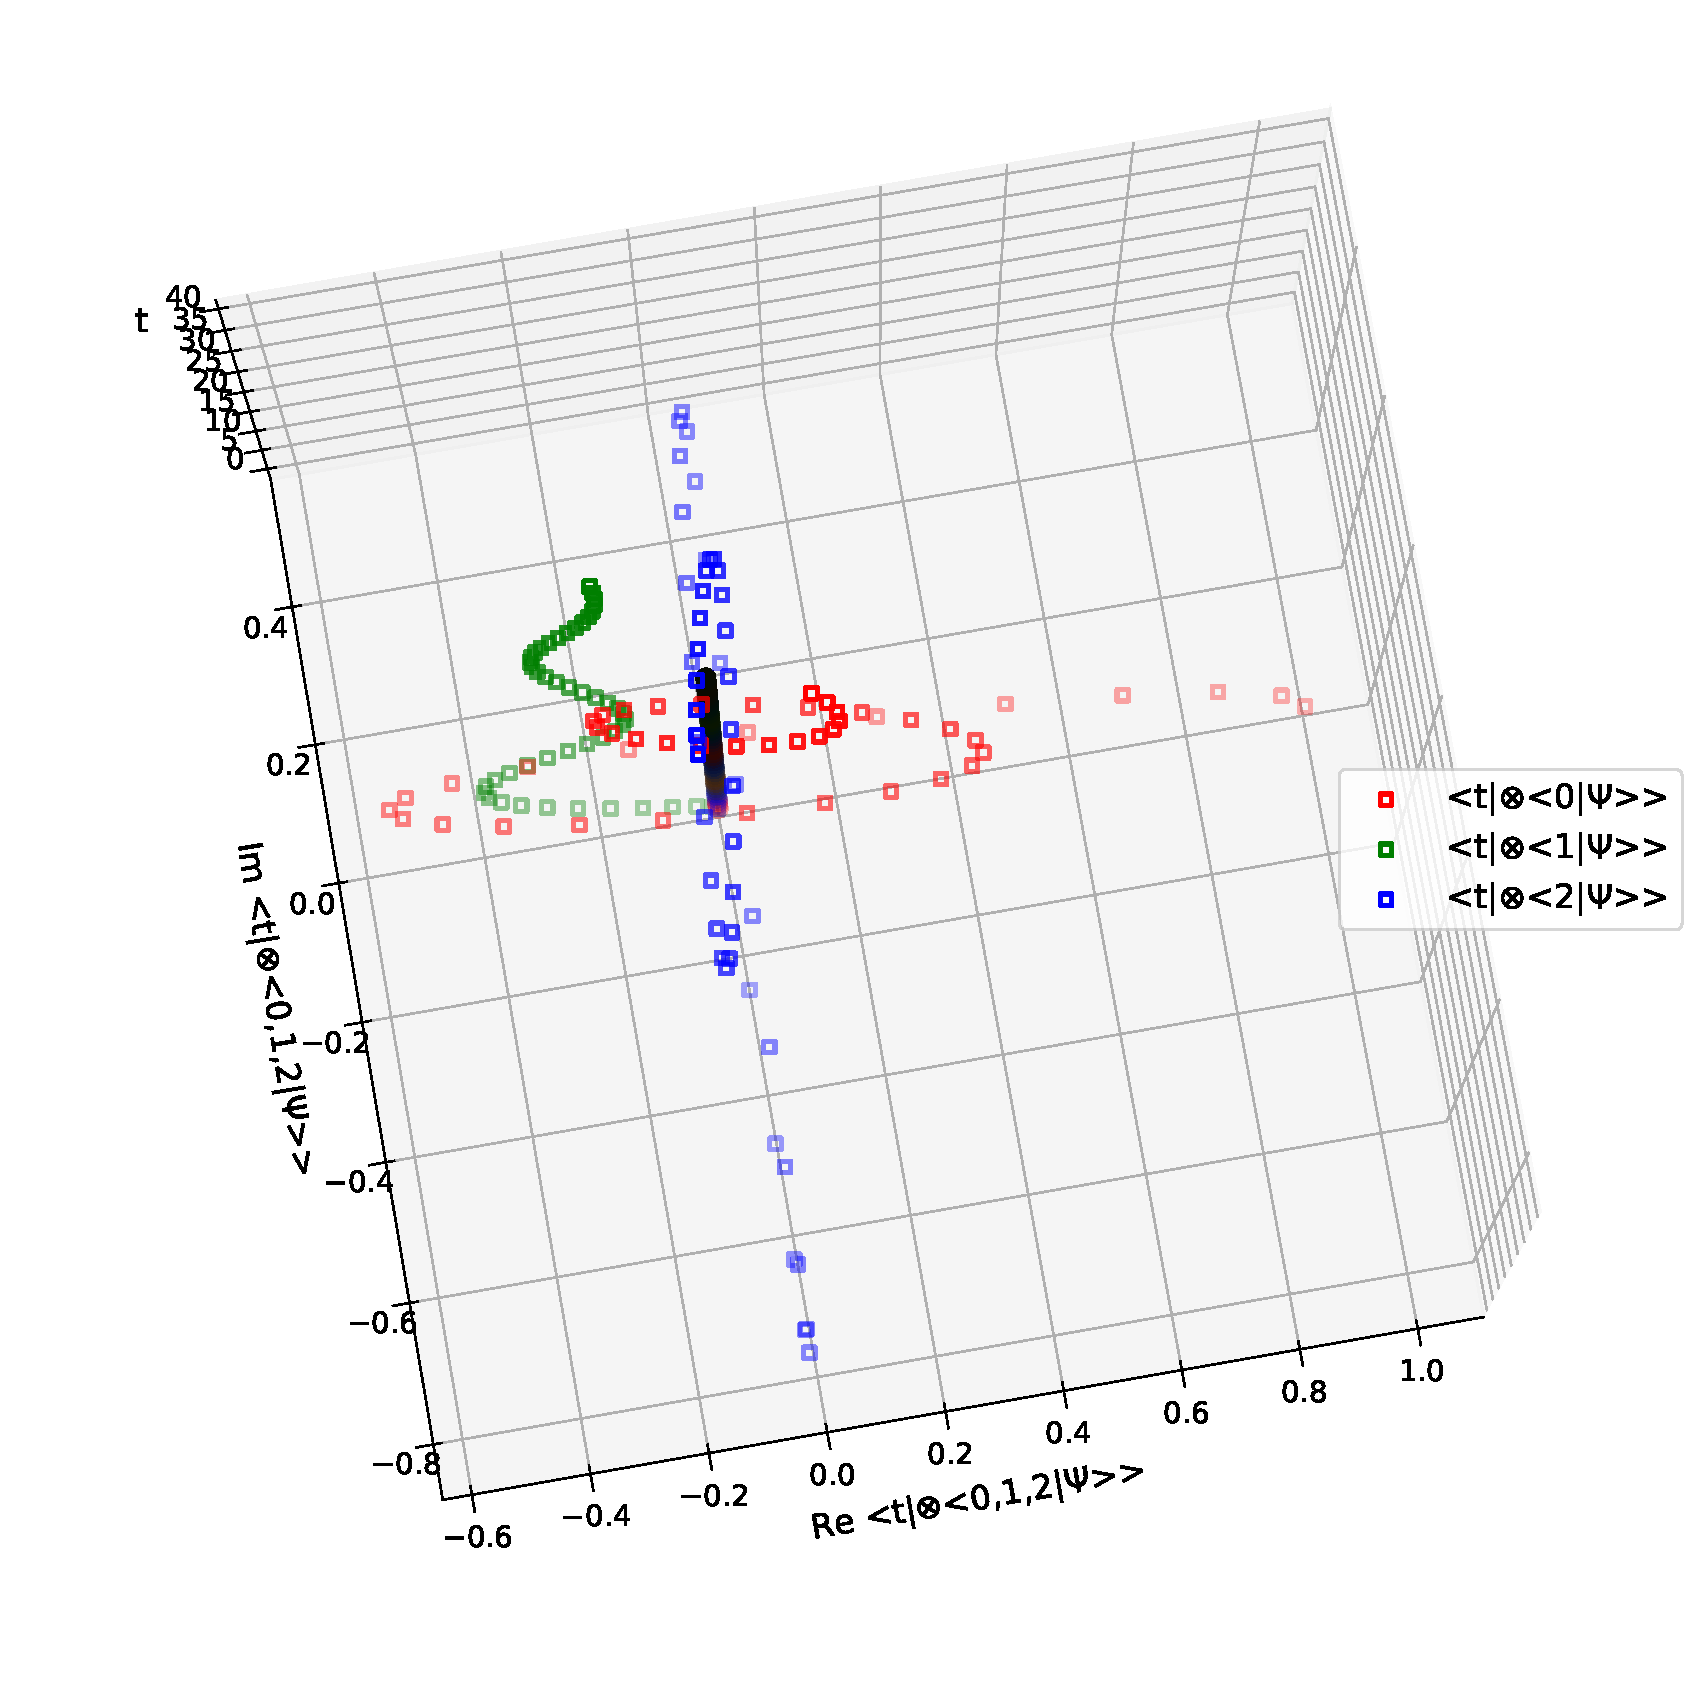
\includegraphics[height=0.48\textheight,clip,trim= 0 60 0 100]{img/3ldetect/PWSpaceTime_top.pdf}
    \caption{3-D plot: top view.}
  \end{subfigure}
  \caption[
    Components (complex values) of $\dket{\Psi} \in \pwspace$
  ]{
    Components (complex values) of the discrete-Page--Wootters vector
    $\dket{\Psi} \in \pwspace$
    (``evolution without evolution'').
    Can be compared with Fig.~\ref{fig:3lev:nonHermitianEvol}.
  }
  \label{fig:3lev:PWSpaceTime}
\end{figure}

% Uses dpfloat and \ContinuedFloat
\begin{figure}[p] % will be the left-side figure
  \begin{leftfullpage}
    \begin{subfigure}{\textwidth}
      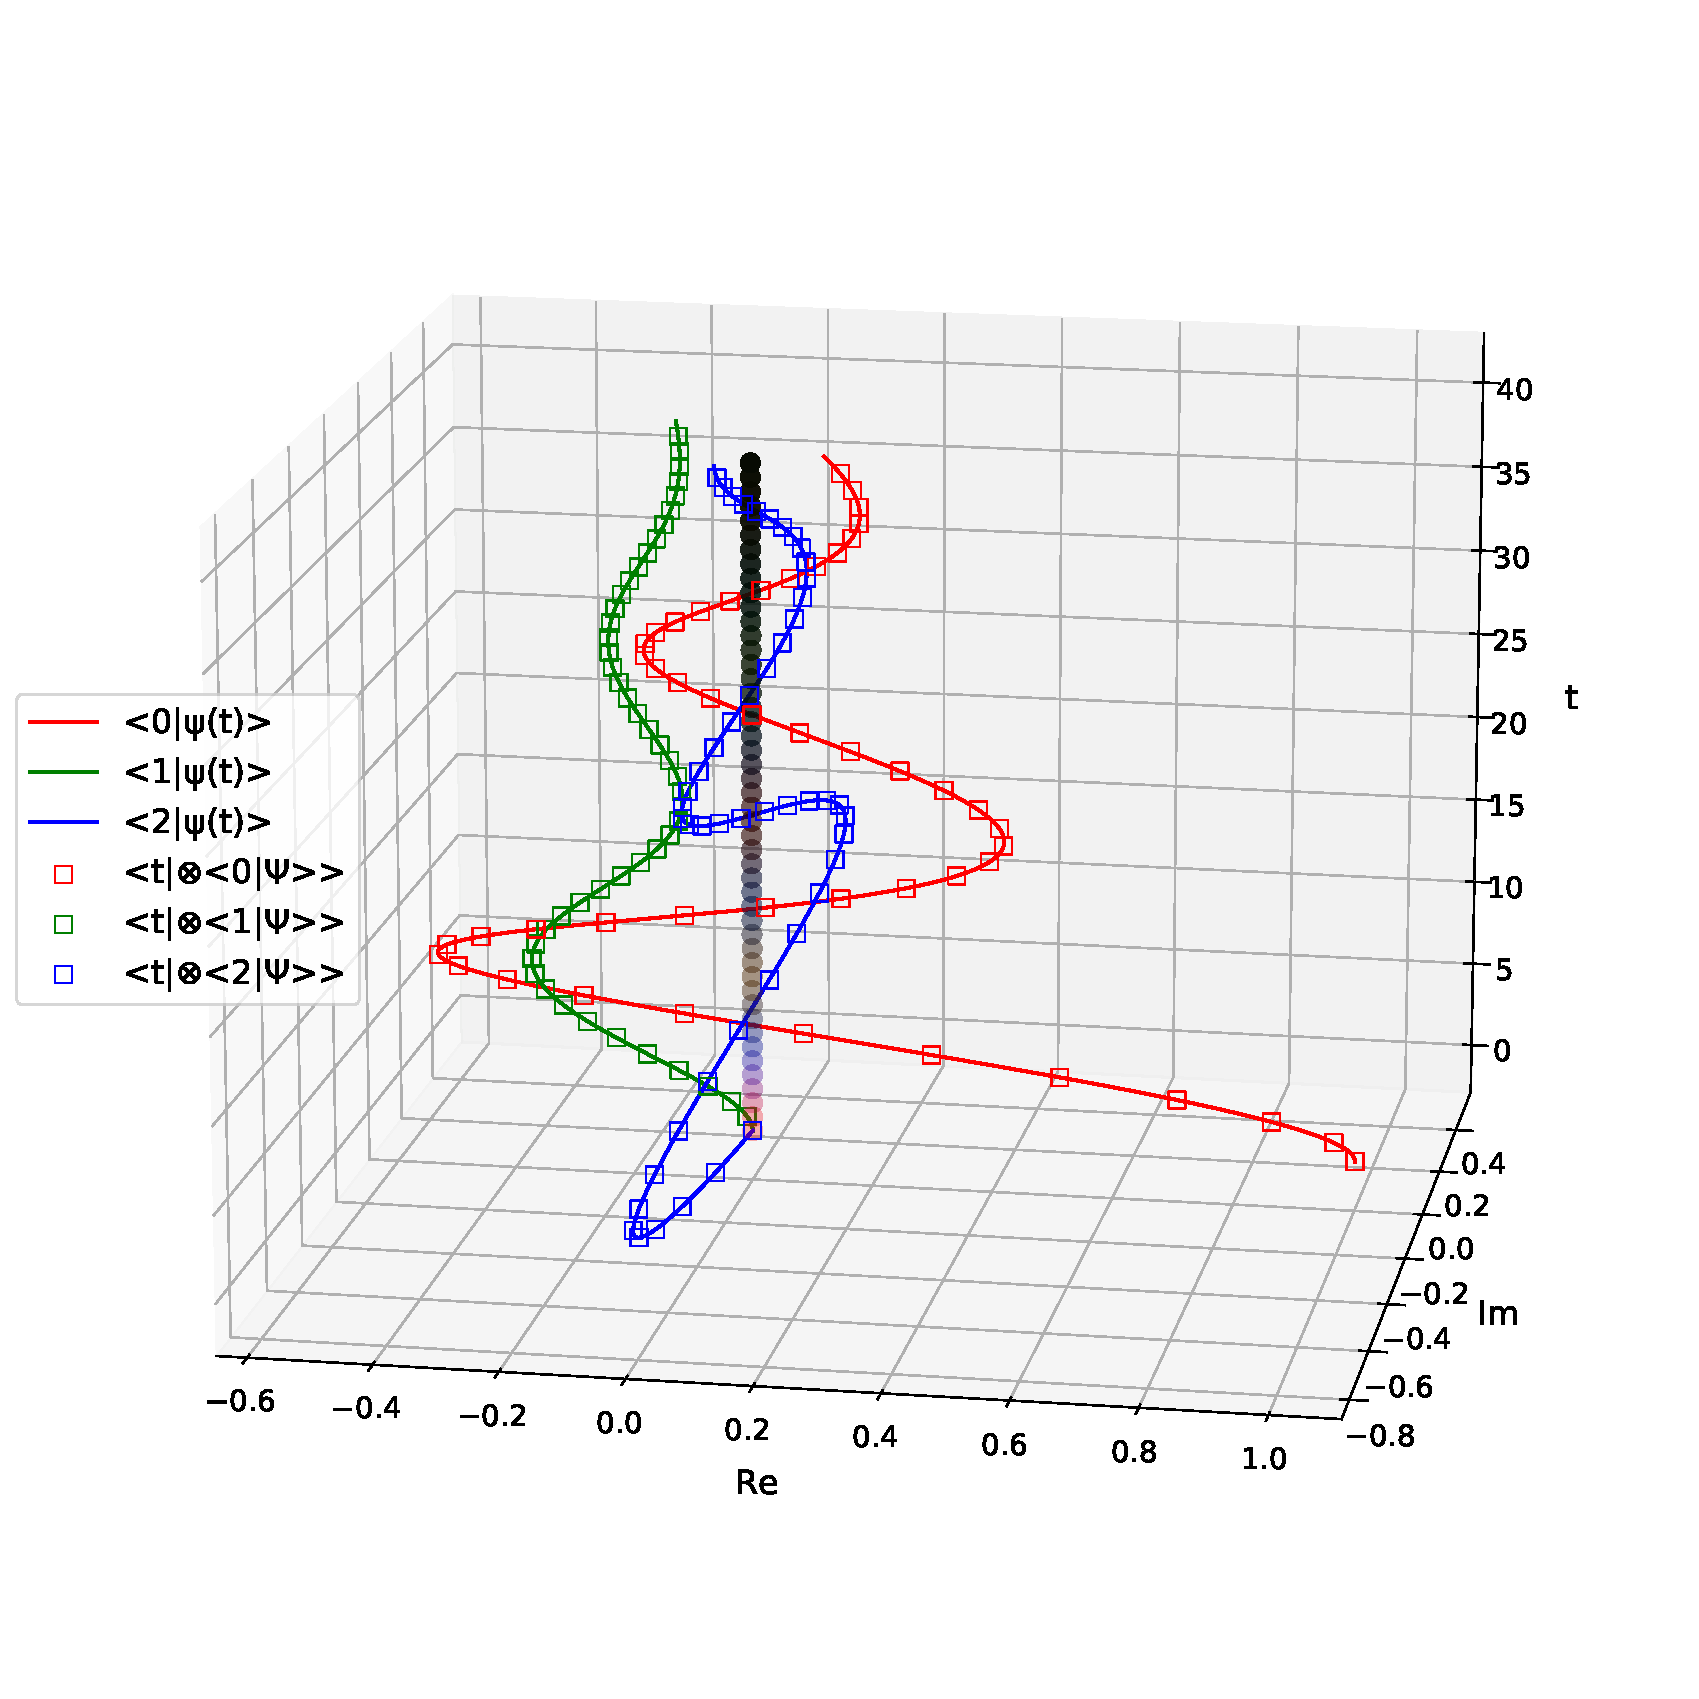
\includegraphics[width=\textwidth]{img/3ldetect/PWSpaceTimeFit_side.pdf}
      \subcaption{3-D plot: side view}
      \label{fig:3lev:PWSpaceTimeFit:side}
    \end{subfigure}
    \caption{
      Discrete Page--Wootters results (points)
      compared to continuous
      Schr\"{o}dinger
      evolution (continuous lines).
    }
    \label{fig:3lev:PWSpaceTimeFit}
  \end{leftfullpage}
\end{figure}
\begin{figure}[p]\ContinuedFloat % will be the right-side figure
  \begin{fullpage}
    \begin{subfigure}{\textwidth}
      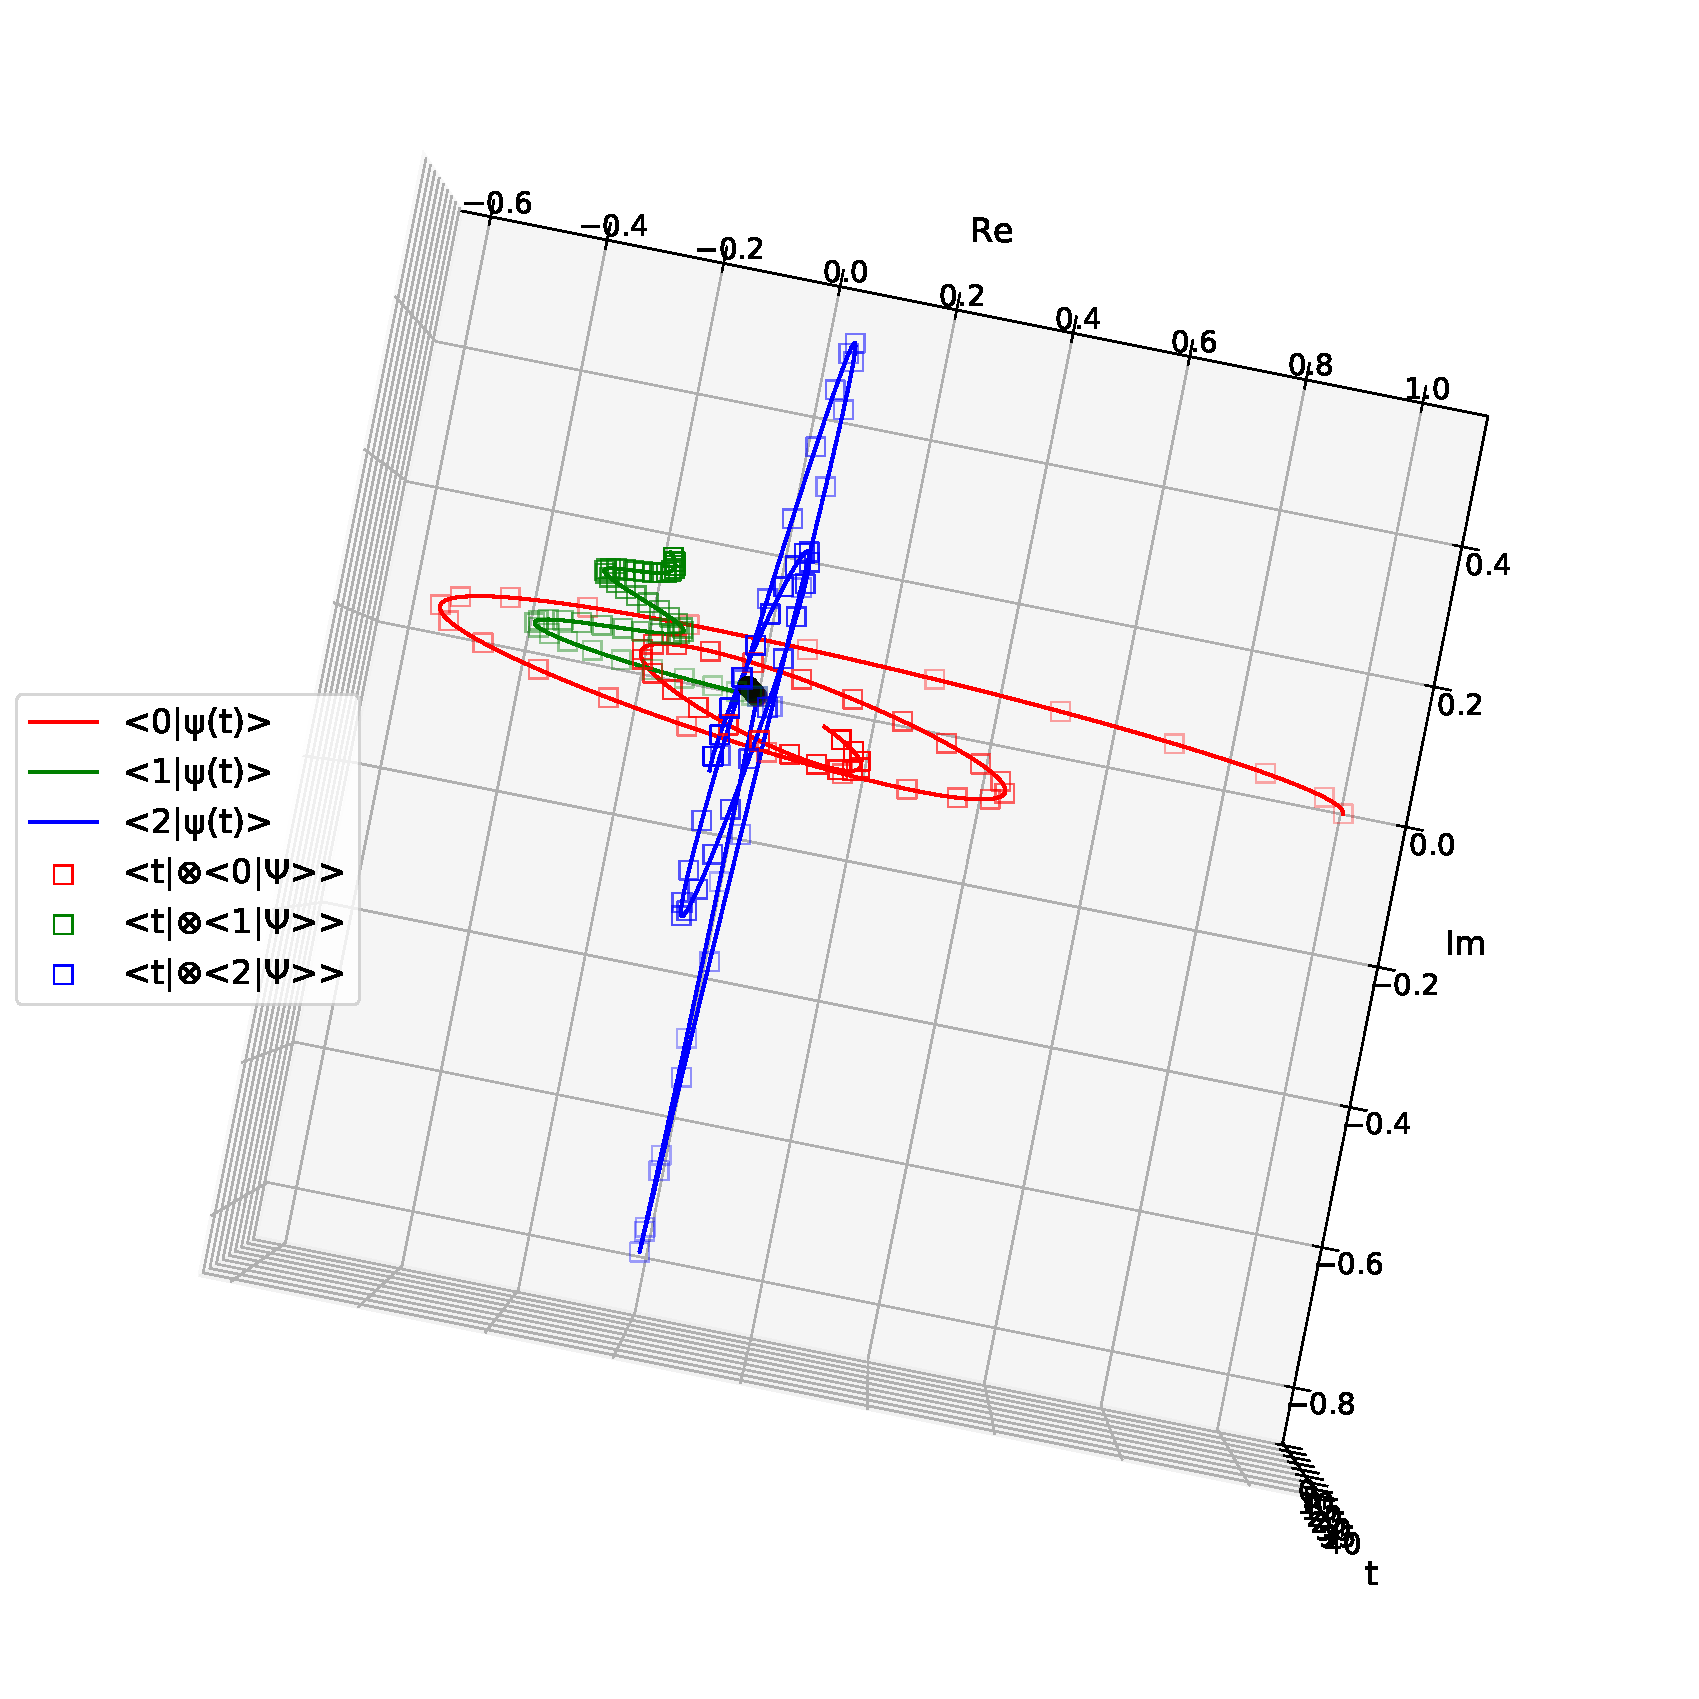
\includegraphics[width=\textwidth]{img/3ldetect/PWSpaceTimeFit_top.pdf}
      \subcaption{3-D plot: top view}
      \label{fig:3lev:PWSpaceTimeFit:top}
    \end{subfigure}
    \caption{
      \textit{Continued from Fig.~\ref{fig:3lev:PWSpaceTimeFit:side}}.
      Discrete Page--Wootters results (points)
      compared to continuous
      Schr\"{o}dinger
      evolution (continuous lines).
    }
  \end{fullpage}
\end{figure}

\subsection{Time-of-arrival (conditional) probability}

From \cite{Maccone:QMOT}, a time-of-arrival probability distribution can be derived
for the three-level system at hand, within the Page--Wootters formalism.
In a finite-dimensional
Hilbert space there's no notion of position or ``region of space'', but, as stated in the
same paper,
\begin{quote}
  [\dots] the whole discussion can be easily extended to the “time at which any
  event happens”. For example, if one considers a spin instead of a particle on a line, one can define the “time at
  which the spin is up”.
  
  [\dots] the notion of ``event'' in quantum mechanics [can be] defined as ``something that happens to a
  quantum system'', where ``something'' means ``a system
  observable property taking some value [\dots]''.
\end{quote}
Rather than spin up or down, in the present example, the arrival time at level $\ket{2}$
can be derived:
\begin{multline}\label{eq:3lev:bayesPW}
  P^{PW}(t_n|2) \eqbydef P^{PW}\Big( t_n \Big| 2, \left[0,\Delta{T}\right]\Big) = \frac{
    \abs{\bra{t_n} \ox \bra{2} \cdot \dket{\Psi}}^2
  }{
    \sum_{n'=0}^{N_{T} - 1} \abs{\bra{t_{n'}} \ox \bra{2} \cdot \dket{\Psi}}^2
  }
  \,\text{,}
  \\
  \text{ where } t_{n'} = n'\delta{T} = \frac{n'\Delta{T}}{N_{T}}
  \text{;}
\end{multline}
which gives the (conditional, \term{Bayesian}) probability that, given that a detection of $\ket{2}$
happens
within $t \in [0, \Delta T]$, it happens at time $t_n$ (or, more correctly, between $t_n$ and $t_{n+1}$).

On the other hand, and outside the Page--Wootters formalism,
within  the absorptive detector model
(see e.g. Sec.~\ref{sec:3lev:complexPotential} or Fig.~\ref{fig:3lev:loss})
the detection probability density reads $p(t) = - \dv{\norm{\psi}^2}{t}$.

Thus, the \emph{conditional} probability density that
---\emph{provided }a detection\footnote{
  Or measurement of related observable eigenvalue,
  or spontaneous decay from $\ket{2}$ as in Sec.~\ref{sec:detect:atomlaser}.
}
of the system at $\ket{2}$ happens within $t \in [0, \Delta{T}]$---
it does happen at a particular time $t$ is
\begin{equation}\label{3lev:condProb}
  p(t|2) \eqbydef p\big(t   \:\big|\:   2,[0,\Delta{T}]\big)
  =
  \frac{
    - \dv{\norm{\psi}^2}{t}
  }{
    \int_{0}^{\Delta{T}} - \dv{\norm{\psi}^2}{t'} \dd{t'}
  }
  =
  \frac{
    - \dv{\norm{\psi}^2}{t}
  }{
    \norm{\psi(0)}^2 - \norm{\psi(\Delta{T})}^2
  }
  \;\text{.}
\end{equation}

The ``state of arrival'' in \eqref{3lev:condProb} is $\ket{2}$
because the operator
in \eqref{eq:3lev:nonUnitaryH:antiHermitianTerm}
is essentially $\op{D} = \gamma \ketbra{2}$. The same
state has been chosen in \eqref{eq:3lev:bayesPW}
to allow a comparison. However, $P^{PW}(t_n|2)$ is a probability,
while $p(t|2)$ is a probability \emph{density}.
Therefore, the \eqref{eq:3lev:bayesPW} should be divided by $\delta T$,
i.e. the duration of the time interval the probability refers to,
before being plotted in Fig~\ref{fig:3lev:condProb},
where the two models show indeed fully compatible results.
\begin{figure}[]
  \centering
  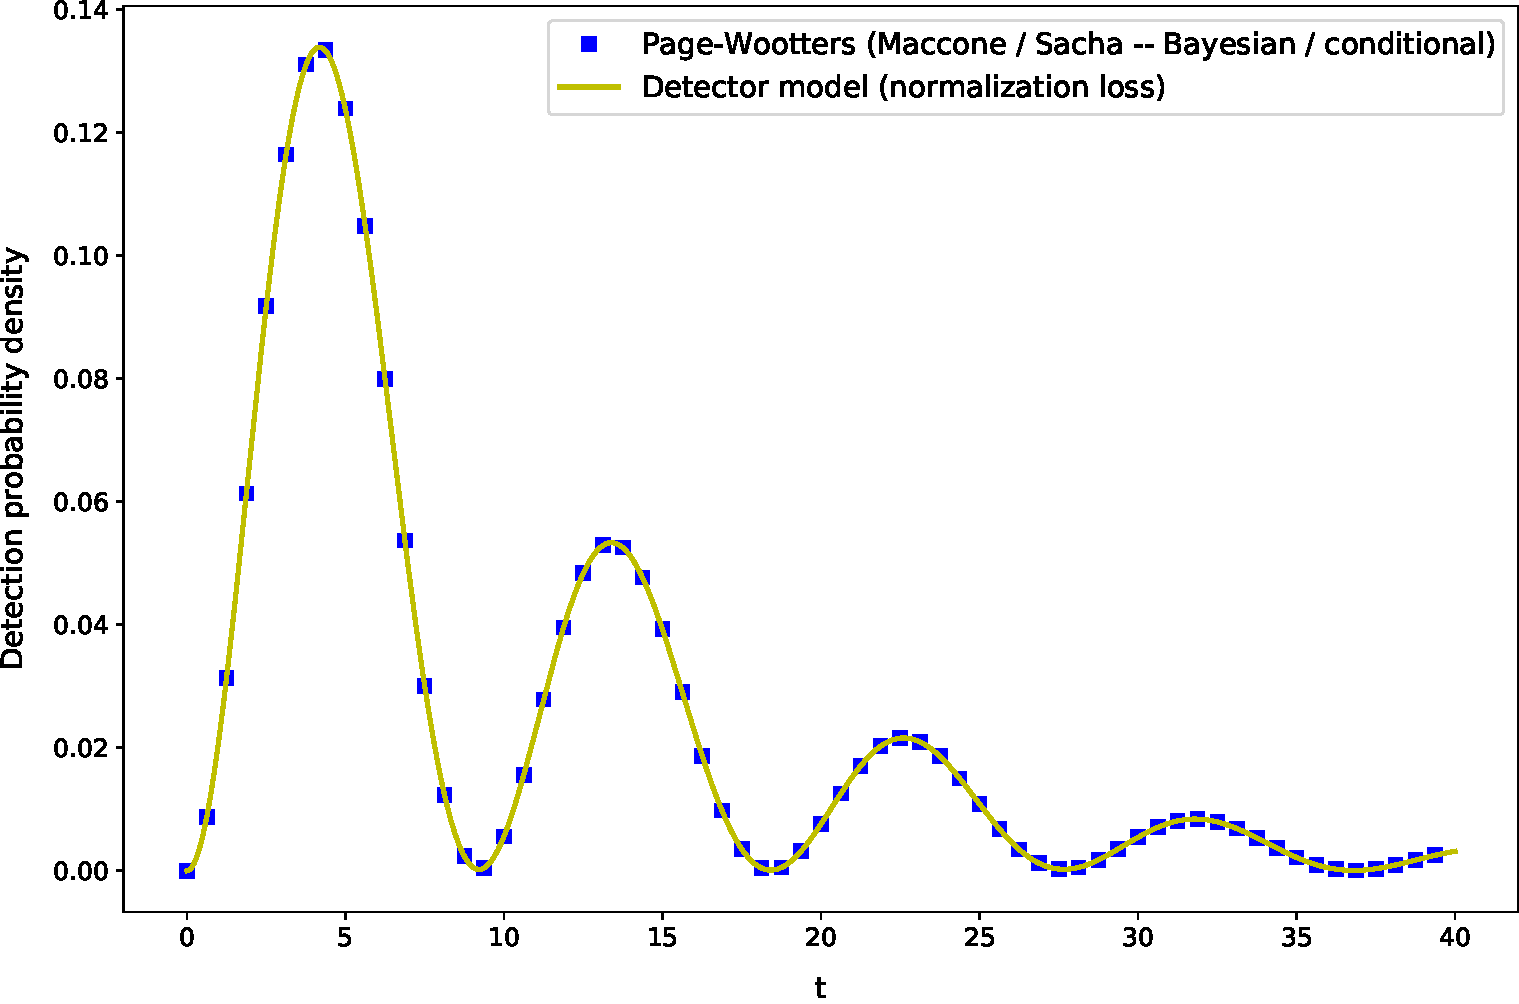
\includegraphics[width=\textwidth]{img/3ldetect/conditionalProbFit.pdf}
  \caption[
    Conditional probability density for time of arrival at state $\ket{2}$.
  ]{
    Conditional probability density for time of arrival at state $\ket{2}$.
    Discrete points: $P^{PW}(t_n|2) / \delta{T}$ (Page--Wootters).
    Continuous line: $p(t|2)$ (detector model).
  }
  \label{fig:3lev:condProb}
\end{figure}

\subsubsection*{\term{NumPy} code}

Relevant portion of code to compute the \eqref{eq:3lev:bayesPW} follows.
Values of probability density
$\frac{1}{\delta{T}}  P^{PW}(t_n|2)$
are stored in the array \Verb|Y|:
\begin{lstlisting}[language=Python]
# [...]
def tn_ox_arrived(n):
  # tensor product
  return np.kron(t_eigenstate(n), arrived_state)

history_normalized = history / norm(history)  ## normalized in H_T \otimes H_S

def joint_prob(n):
  return np.abs(tn_ox_arrived(n) @ history_normalized)**2

X = np.arange(NT)
iterable = (joint_prob(n) for n in X)
Y = np.fromiter(iterable, float)
dT  = DT / (NT)

# A "time bin"
X = X * dT # real time
Y = Y / dT # probability _density_

bayes_denominator = np.sum(Y * dT)
Y = Y / bayes_denominator
\end{lstlisting}

The \eqref{3lev:condProb} is partly implemented
directly in the plotting code:
\begin{lstlisting}[language=Python]
ax.plot(times, -np.gradient(norms**2, times) / bayesian_denominator_nonpw,
c='y', linewidth=2, label='Detector model (normalization loss)')
\end{lstlisting}
particularly with the expression
\lstinline{-np.gradient(norms**2, times) / bayesian_denominator_nonpw}.
The array \Verb!norms! was previously assigned values of $\norm{\psi(t)}$
while computing the non-unitary evolution for the problem in Sec.~\ref{sec:3lev:complexPotential}.
Here, explicitly:
\begin{lstlisting}[language=Python]
# [...]
def B(_t, _gamma=GAMMA):
  return expm(-1j*K(_gamma)*_t)

def non_unitary_psi(_t, _gamma=GAMMA):
  return B(_t, _gamma) @ psi_0

# [...]
_iter_norm = (norm(non_unitary_psi(_t)) for _t in times)
norms = np.fromiter(_iter_norm, np.float)
\end{lstlisting}
where, again, the function \Verb!K()! returns the matrix in \eqref{eq:3lev:nonUnitaryH}.
As per the ``Bayesian denominator'':
\begin{lstlisting}[language=Python]
# loss of normalization, or integral of antiderivative...
bayesian_denominator_nonpw = 1 - norm(evolution.T[NPLOTPOINTS-1])**2
\end{lstlisting}

Full code for this Section can be consulted at Appendix \ref{toa-prob-as-in-macconesacha-arxiv1810.12869}.
